\documentstyle[times]{acmconf}
\input{/group/csdl/tex/psfig/psfig}

\begin{document}

\title{Investigating Data Quality Problems in the PSP \\ \par \medskip 
       {\small Experience Paper}}

\author{
        Anne M. Disney\\
        Philip M. Johnson
        Dept. of Information and Computer Sciences\\
        University of Hawaii\\
        Honolulu, HI  96822 USA\\
        anne@ics.hawaii.edu\\
        johnson@hawaii.edu}
       }

%\toappearbox{Submitted to the Sixth International Symposium on the
%Foundations of Software Engineering (FSE-6), Orlando, Florida, November, 1998.}

\maketitle

%PJ -- abstract modified
\begin{abstract}
  
  The Personal Software Process (PSP) is used by software engineers to
  gather and analyze data about their work.  Published studies typically
  use data collected using the PSP to draw quantitative conclusions about
  its impact upon programmer behavior and product quality.  However,
  our experience using PSP in both industrial and academic settings
  revealed problems both in collection of data and its later analysis.
  We hypothesized that these two kinds of data quality problems could make a
  significant impact upon the value of PSP measures.  To test this
  hypothesis, we built a tool to automate the PSP and then examined 89
  projects completed by ten subjects using the PSP manually in an
  educational setting.  We discovered 1539 primary errors and categorized
  them by type, subtype, severity, and age.  To examine the collection
  problem we looked at the 90 errors that represented impossible
  combinations of data and at other less concrete anomalies in Time
  Recording Logs and Defect Recording Logs.  To examine the analysis
  problem we developed a rule set, corrected the errors as far as possible,
  and compared the original and corrected data.  This resulted in
  significant differences for measures such as yield and the
  cost-performance ratio, confirming our hypothesis.  Our results raise
  questions about the accuracy of manually collected and analyzed PSP data,
  indicate that integrated tool support may be required for high quality
  PSP data collection and analysis, and suggest that external measures
  should be used when attempting to evaluate the impact of the PSP.

\end{abstract}

\subsection*{Keywords}

\noindent Personal software process, defects, 
empirical software engineering,
measurement dysfunction, automated process support\\


%%%%%%%%%%%%%%%%%%%%%%%%%%%%%% -*- Mode: Latex -*- %%%%%%%%%%%%%%%%%%%%%%%%%%%%
%% intro.tex -- 
%% Author          : Carleton Moore
%% Created On      : Fri Oct 18 16:20:55 1996
%% Last Modified By: Carleton Moore
%% Last Modified On: Wed Nov 20 16:41:34 1996
%% RCS: $Id: intro.tex,v 1.4 1996/11/21 02:42:55 cmoore Exp $
%%%%%%%%%%%%%%%%%%%%%%%%%%%%%%%%%%%%%%%%%%%%%%%%%%%%%%%%%%%%%%%%%%%%%%%%%%%%%%%
%%   Copyright (C) 1996 Carleton Moore
%%%%%%%%%%%%%%%%%%%%%%%%%%%%%%%%%%%%%%%%%%%%%%%%%%%%%%%%%%%%%%%%%%%%%%%%%%%%%%%
%% 

\section{Introduction}
\label{sec:intro}

\subsection{Motivation}

\subsection{Theses}
\begin{enumerate}
\item {An appropriately designed computer-mediated formal technical review
    environment will be adopted in an industrial environment and will yield
    substantial improvements in measures of review efficiency and
    effectiveness without introducing metrics dysfunction.}

\item {The AFTR technology transfer method's instrumentation will provide valuable
    insights into the strengths and weaknesses of this technology transfer
    method.}

\end{enumerate}

\subsubsection{Hypotheses}
\begin{enumerate}
\item[H1.1:]{There will be observable differences in review
effectiveness between the manual process and the automated process.}
\item[H1.2:]{There will be a observable difference in cost between
the manual FTR process and the automated FTR process.}
\item[H1.3:]{The organization will adopt AFTR as their FTR tool.}
\item[H1.4:]{The participants will prefer to use the automated FTR
process over the manual FTR process.}
\item[H2.1:]{Analysis of the process defects will lead to Process
Improvement Proposals (PIPs).}
\item[H2.2:]{Process Improvement Proposals (PIPs) from the method will
provide insight to improving the technology transfer method.}
\end{enumerate}

\subsubsection{Research Questions}
\begin{itemize}
\item{How do we develop a system that measures FTR without introducing
dysfunction?}
\item{Does a system that measures FTR without introducing dysfunction,
provide management with the answers they want?}
\item{Will a FTR system without dysfunction be adopted?}
\end{itemize}

\subsubsection{Definition of Improvement:}
\begin{itemize}
\item{less effort}
  \begin{itemize}
  \item{overall time spent in TekInspect}
  \item{individuals spend less time doing AFTR than TekInspect}
  \item{less rework time per defect}
  \item{reduces scribe's work}
  \item{makes group meetings more effective}
  \end{itemize}
\item{more defects found}
  \begin{itemize}
  \item{allows reviewers to focus on review not process}
  \item{more severe errors than minor}
  \item{defects per hour goes up}
  \end{itemize}
\item{participants like new automated system}
  \begin{itemize}
  \item{participants feelings toward FTR improves}
  \item{participants want to have their work reviewed}
  \item{Esprit de corps}
  \item{team building}
  \end{itemize}
\item{more groups use FTR with AFTR than with out}
  \begin{itemize}
  \item{number of groups using TekInspect vs AFTR}
  \item{more groups asking to use AFTR}
  \end{itemize}
\item{Management sees benefits of FTR from AFTR}
  \begin{itemize}
  \item{cost savings}
  \item{more predictability for reviews using AFTR}
  \item{reduced time for projects using AFTR}
  \item{Management want teams to use AFTR}
  \end{itemize}
\end{itemize}

This proposal is organized as following: Section \ref{sec:related} relates
the current research to the broader context of existing work.  Section
\ref{sec:method} introduces our method for introducing automated FTR into
an organization.  Section \ref{sec:manual} describes the manual FTR method
being used.  Section \ref{sec:AFTR} depicts the main design features and
architecture of AFTR.  Section \ref{sec:experiment} outlines the
experimental case study I plan to conduct to evaluate AFTR.  Finally,
Section \ref{sec:plan} presents the current research plan.


%%%%%%%%%%%%%%%%%%%%%%%%%%%%%% -*- Mode: Latex -*- %%%%%%%%%%%%%%%%%%%%%%%%%%%%
%% overview.tex -- 
%% Author          : Philip Johnson
%% Created On      : Wed Apr  8 14:23:39 1998
%% Last Modified By: Philip Johnson
%% Last Modified On: Mon Aug 10 14:36:38 1998
%% RCS: $Id$
%%%%%%%%%%%%%%%%%%%%%%%%%%%%%%%%%%%%%%%%%%%%%%%%%%%%%%%%%%%%%%%%%%%%%%%%%%%%%%%
%%   Copyright (C) 1998 Philip Johnson
%%%%%%%%%%%%%%%%%%%%%%%%%%%%%%%%%%%%%%%%%%%%%%%%%%%%%%%%%%%%%%%%%%%%%%%%%%%%%%%
%% 

\section{OVERVIEW OF THE PSP}


In the PSP curriculum presented in ``A Discipline for Software
Engineering'', each student develops 10 small programs over the course of a
semester using a sequence of seven increasingly sophisticated software
development processes, labeled PSP0 to PSP3.  For every program, the students record various
measurements related to their personal development activities. Such
measures include, for example, the time spent in each phase of development,
the numbers of defects injected and removed during each phase, and the size
of the resulting work product.

The initial programs use relatively simple processes that establish a
baseline set of process measures for time, size, and defects. Later
programs employ more advanced processes that extend these baseline
process statistics.  Although there are a myriad of individual extensions, 
most fall into two conceptual categories.

First, the planning phase is expanded to include estimates of the program's
projected size, the projected time required to complete each of the phases,
and the number of anticipated defects that will be injected and removed
during development.  The process by which these estimates are produced
involves statistical analysis of historical correlations between designs
(i.e. class and method counts) and actual size (in lines of code), between
estimated size and actual time, between actual size and actual time, and
between size and defects injected and removed.  (While lines of code as a
metric of size at the organizational level is almost uniformly excoriated
in the measurement literature, it seems to work surprisingly well in the
PSP, since the measure is collected and applied to a single individual working
in a single language in a relatively uniform domain.)

Second, by the middle of the course, each student has typically recorded a
hundred or more defects made during development.  Later processes
include mechanisms to help students understand the impact of various kinds
of defects and to drive process improvements intended to reduce future
occurrence of important defect types. For example, since students record
the phase each defect was injected and removed and the time required to fix
it, it is possible to analyze the relationship between fix time and various
characteristics of defects.  One relationship nearly
always present in student data is that the ``longer'' a defect is present,
the more time it takes to remove it.  Thus, defects injected during design
and not removed until testing are nearly always more expensive to remove
than, for example, defects injected during coding and removed during
compiling. This outcome typically motivates students to put more effort and
care into design activities. Later processes support such behaviors by
providing active defect management mechanisms. For example, by analyzing
defect data to determine the types of design defects made on prior
projects, a student can generate a checklist to be used as part of a
personal design review to ensure that those defects do not escape into
code, compile, or test phases.

The final stages of the course further extend the basic PSP para\-digm.  The
last PSP process provides a way to scale the method to support larger
projects using a cyclic development method. In addition, PSP includes a
meta-level process for defining personal processes in non-software domains
or for specific software organizational contexts.


%%%%%%%%%%%%%%%%%%%%%%%%%%%%%% -*- Mode: Latex -*- %%%%%%%%%%%%%%%%%%%%%%%%%%%%
%% problems.tex -- 
%% Author          : Philip Johnson
%% Created On      : Wed Apr  8 14:23:59 1998
%% Last Modified By: Philip Johnson
%% Last Modified On: Mon Aug 10 14:19:37 1998
%% RCS: $Id$
%%%%%%%%%%%%%%%%%%%%%%%%%%%%%%%%%%%%%%%%%%%%%%%%%%%%%%%%%%%%%%%%%%%%%%%%%%%%%%%
%%   Copyright (C) 1998 Philip Johnson
%%%%%%%%%%%%%%%%%%%%%%%%%%%%%%%%%%%%%%%%%%%%%%%%%%%%%%%%%%%%%%%%%%%%%%%%%%%%%%%
%% 

\section{A MODEL OF PSP DATA QUALITY}

\begin{figure*}
%   {\centerline{\psfig{figure=graphic2.eps}}}
    {\centerline{\psfig{figure=PSPmodel.eps}}}
    \caption{\label{fig:model} A simple model for PSP data quality. Through 
      a process of {\em collection}, the developer generates an initial
      empirical representation (``Records of Work'') of her personal process
      (``Actual Work'').  Through additional {\em analyses}, the developer
      augments her initial empirical representation with
      derived data (``Analyzed Work'') intended to enable process improvement
      through ``Insights about Work''.
      }
\end{figure*}
     
To guide our understanding of data quality problems in the PSP, we devised
a simple two stage model of PSP data, as illustrated in Figure
\ref{fig:model}.  The model begins with ``Actual Work''---the actual developer
efforts devoted to a software development project.  As part of these
efforts, the developer {\em collects} a set of primary measures on defects,
time, and work product characteristics---the ``Records of Work''. Based on
these primary measures, the developer performs additional {\em analyses},
many of which result in secondary (i.e.  derived) measures which are
themselves inputs for further analyses.  The secondary, derived measures
and associated analyses are presented in various PSP forms---the ``Analyzed
Work''---and hopefully yield ``Insights about Work'' to improve future
software development activities.

% Added by AD, 08/06/98
We based this model upon the PSP as presented in {\it A Discipline for
  Software Engineering} \cite{Humphrey95}
--- what we term ``manual PSP''.  
Manual PSP refers to a situation in which the PSP forms must be filled out
by hand, either by editing a copy of the form on-line, or by filling out
out a printed copy with pen or pencil.  Even if tools such as spreadsheets
are used to collect historical data and to provide various computations, if
they do not automatically insert and maintain the correct calculated values
in the appropriate places in the forms, then we define the technique as
``manual''.  We define partially or fully ``automated'' PSP as one in which 
some or all of the derived measures are calculated and placed into the forms
automatically.  In other words, in automated PSP, the analysis tools and
forms presenting the PSP reports are tightly {\it integrated}. 
Although ``automated'' PSP can essentially automate all of the analysis stage
calculations, there are limits to its ability to automate the collection
stage work.  The collection stage is still quite ``manual'' in nature.

At the time we performed this case study, there was no {\em integrated}
software support for the PSP.  Thus, the case study employed what we call the
``manual'' version of the PSP, despite our extensive use of spreadsheets, program
size counting tools, and statistical tools during the course.  Since then,
integrated tools have become available, including spreadsheets available at
the Addison-Wesley FTP site which print out the project summary forms, and
the Personal Software Process Studio tool produced by East Tennessee State
%PJ
University \cite{PSPS97}.
% end add by AD

There are three basic ways to affect PSP data quality in the collection
stage: errors of omission, errors of addition, and errors of transcription.
Errors of omission occur when the developer does not record a primary
measure related to defects, time, or the work product itself.  If a defect
occurring during ``Actual Work'' does not appear in the ``Records of Work'', then, for
example, the PSP model of that work product's defect density will be lower
than its actual defect density. If time spent on the work product is not
recorded, then the PSP model of that developer's productivity will be
higher than her actual productivity. Errors of addition occur when the
developer augments the ``Records of Work'' with data not reflecting
actual practice. For example, a developer, having made an error of omission
to the point of having no time or defect data, may recover by simply
inventing enough time and defect entries to make his or her PSP data appear
plausible. Finally, errors of transcription occur when the developer does
intend to record their ``Actual Work'' in the ``Records of Work'' but makes a
mistake during this process.

The presence of collection stage data quality problems is typically
difficult to ascertain and difficult or impossible to rectify. In the
PSP, primary data collection often feels both time consuming and
psychologically disruptive.  Many students complain that stopping to record
defects disrupts their ``flow'' state, and that the time spent recording a
defect---particularly for compilation stage errors---often exceeds the time
spent correcting the defect.  The PSP requires users to learn to constantly
interleave ``doing work'' with ``recording what work you are doing''.

There are also three basic ways to affect PSP data quality in the analysis
stage of manual PSP: errors of omission, errors of calculation, and errors of
transcription.  Errors of omission occur when the developer does not
perform a required analysis of the primary data. Errors of calculation
occur when the developer attempts to perform an analysis but does so
incorrectly. For example, a developer might use a regression-based
estimation method when the historical data is so uncorrelated that this
method is invalid. Finally, errors of transcription occur when the
developer makes a clerical error when moving data from one form to another.

Unlike the collection stage, analysis stage data quality problems are much
easier to ascertain and correct, {\em provided that errors did not occur
  during the collection stage}.  In other words, if one assumes that the
work records accurately reflect the underlying work, then appropriate use
of automated tools can reduce or eliminate analysis errors of
omission, calculation, and transcription.  On the other hand, since the
quality of these analyses are totally dependent upon the quality of the
work records, overall PSP data quality could be quite low even if the
analysis stage is totally automated to eliminate all of its potential data
quality errors.







 
%%%%%%%%%%%%%%%%%%%%%%%%%%%%%% -*- Mode: Latex -*- %%%%%%%%%%%%%%%%%%%%%%%%%%%%
%% case-study.tex -- 
%% Author          : Philip Johnson
%% Created On      : Wed Apr  8 14:24:28 1998
%% Last Modified By: Philip Johnson
%% Last Modified On: Mon Aug 10 14:26:51 1998
%% RCS: $Id$
%%%%%%%%%%%%%%%%%%%%%%%%%%%%%%%%%%%%%%%%%%%%%%%%%%%%%%%%%%%%%%%%%%%%%%%%%%%%%%%
%%   Copyright (C) 1998 Philip Johnson
%%%%%%%%%%%%%%%%%%%%%%%%%%%%%%%%%%%%%%%%%%%%%%%%%%%%%%%%%%%%%%%%%%%%%%%%%%%%%%%
%% 3 pages


\section{CASE STUDY}

To gain insight into the occurrence and significance of collection and
analysis data quality problems, we conducted a case study. The case study
began by teaching a modified version of the PSP designed to improve data
quality.  Next, we entered the data into a database that automated most
analysis calculations and revealed the presence of a subset of the possible
errors in student data.  We then performed additional analyses on these
errors to understand their cause and potential significance to PSP data
values and the method itself.

  \subsection{The Modified PSP Curriculum}
  
  The projects used for this study were obtained from a software
  engineering class taught by Philip Johnson, in which the PSP was taught
  over the course of a semester using nine project assignments. There were
  ten students in the class, and 89 completed projects.
   
  Because of the concern with data quality from prior experience teaching
  PSP, the instructor made four principal modifications to the standard PSP
  curriculum: increased process repetition,  increased process description,
  technical reviews, and tool support.
  
  {\bf Increased process repetition.} In the standard PSP curriculum,
  students are assigned 10 programs during the semester (in addition to
  several midterm and final reports). Over the course of these ten
  programs, students practice seven different PSP processes, which means
  that the development process used by the students changes for seven out
  of ten programs.  From our initial experience with the PSP, we found
  that the overhead of this almost constant ``process acquisition'' led to
  data errors and had a significant impact upon the overall data values.
  To ameliorate this problem, the modified curriculum included only five
  PSP processes, enabling students to practice most
  processes at least twice before moving on to a new one. The modified
  curriculum also included only nine programs instead of ten, providing
  additional time in each program for data collection and analysis.
  
  {\bf Increased process description.} In our initial experiences teaching
  the PSP, the instructor found that students had a great deal of trouble
  learning to do size and time estimation correctly.  For example, PSP time
  estimation requires choosing between three alternative methods for
  estimation depending upon the types of correlations that exist in the
  historical process data from prior programs.  To help resolve this and
  other problems, the instructor added four additional worksheets: (1) a
  Time Estimating Worksheet to provide a guide through the various methods
  of time estimation; (2) a Conceptual Design Worksheet to help in
  developing class names, method names, method parameters, and method
  return values; (3) an Object Size Category Worksheet to help in size
  estimation; and (4) a Size Estimating Template Appendix to provide a
  place to record planned and actual size for prior projects.
  
  {\bf Technical reviews.} At the completion of each project, students
  divided into pairs and carried out a technical review of each other's
  work.  A two-page checklist facilitated this process.  It included such
  questions as ``Did the author follow the PSP Development Phases
  correctly?'' and ``Is the Projected LOC calculated correctly?''  A second
  ``Technical Review Defect Recording Log'' form included columns for
  number, document, severity, location, and description. Students were
  given approximately 60 minutes to do the review.  The technical review
  forms were submitted with the completed projects.  The instructor
  reviewed the projects a second time for grading purposes, using the
  Technical Review Defect Recording Log to record any additional mistakes.
  
  {\bf Tool support.} Finally, the instructor provided four spreadsheets to
  support records of planned and actual data values. In addition, students
%PJ
  were provided with well-tested tools to count non-comment source lines of
  code for Java programs, to compare two versions of a Java program and
  report non-comment lines of code added and deleted, and to perform
  certain statistical analyses.  (In the textbook PSP curriculum, students
  ``bootstrap'' their environment by implementing these tools themselves.
  While elegant pedagogically, this approach unfortunately introduces a
  potentially significant source of data quality problems, since these
  freshly developed tools with no usage history are used to generate many
  of the measures used in later data analysis.)


%PJ more changes (08/06 Added AD)
  In addition to these curriculum modifications, the instructor
  emphasized data quality throughout the course, as recommended in the
  textbook.  For example, he augmented the lecture notes in the
  Instructor's Guide with fully worked out examples of the PSP process data
  for a fictitious student to show how data is collected and analyzed for
  each assignment and accumulated over the course of the semester.  He
  dedicated lectures to collection and analysis of data periodically
  throughout the semester. He regularly showed the class aggregate
  statistics on class performance.  He met with students individually and
  in groups throughout the semester to go over their assignments and PSP
  data while they were in the midst of planning, design, code, compile,
  test, and/or postmortem; but prior to project turn-in.  He uncovered and
  removed many, many PSP data errors through these meetings which are not
  counted in our results.  He did technical reviews of every assignment's
  PSP data, and circulated problem reports throughout the semester
  summarizing issues discovered from student data.

  \subsection{PSP Data Entry Tool}
  
  We developed a database application to support analysis of PSP data from
  PSP0 to PSP2, using the Progress 4GL/RDBMS \cite{Progress98}.  In order
  to reduce opportunities for making mistakes, this tool was designed to
  require a minimum amount of user input and to provide the user with
  default values whenever possible.  Apart from task and scheduling template 
  values, the application automated all calculations, from determining delta 
  times for Time Recording Log entries to performing linear regression for 
  size estimation. In addition, the application guides the user through the
  appropriate forms and fields in the order most appropriate for the
  current process and phase.
 
  \subsection{Error Recording Method}
  
  Once the database application was ready, we entered data from the student
  project PSP forms manually and compared each student value with the
  value computed by the application.  Although every discrepancy
  between the manually generated data and the application-generated data
  could be considered an error, we only counted an error at its insertion
  point.  For example, in a Time Recording Log entry for the Design phase,
  if {\it Stop} is incorrectly subtracted from {\it Start}, {\it Delta
    Time} will be incorrect.  Even if all other calculations are done
  correctly for the rest of the project, {\it Time in Phase, Design,
    Actual}; {\it Time in Phase, Total, Actual}; {\it Time in Phase,
    Design, To Date}; {\it Time in Phase, Total, To Date}; {\it Time in
    Phase, To Date \%}; and {\it Time in Phase, To Date} values for an
  indefinite number of future projects will all be inaccurate to some
  degree.  And this is just for the most simple process, PSP0!  In more
  advanced processes {\it LOC/Hour}, time estimation, {\it Cost-Performance
    Index}, and {\it Defect Removal Efficiency} values could all be
  affected for both the current project and future projects.  To eliminate
  this combinatorial explosion in the number of errors, we counted this as a
  single error in {\it Delta Time}. 
  
  Although we analyzed the project data quite carefully, we do not feel
  confident that we have uncovered all or even most of the errors in this
  case study.  While our database application does enable us to determine
  the correctness or incorrectness of values generated during the analysis
  stage of our data quality model, it provides only limited insight into
  collection stage errors.  For example, in the Time Recording Log, it was
  possible to check the {\it Delta Time} computation, but not the accuracy
  of {\it Date}, {\it Start}, {\it Stop}, or {\it Interruption Time}.  Of
  course, the tool could not, in general, detect the absence of entries for
  work that was done but not recorded.  Two other areas that created
  similar problems were the Defect Recording Log and the measured and
  counted {\it Program Size} fields for the Project Plan Summary.

  \subsection{PSP Error Data Analysis Tool}
  
  In order to analyze the 1539 errors uncovered by the PSP data entry tool,
  we developed a second database application, the PSP Error Data Analysis
  Tool.  For each error discovered, we tracked the person who made the
  error, the method by which the error was found (technical review,
  instructor review, or comparison with the PSP tool results), the
  assignment in which the error occurred, the PSP process used for that
  assignment, the PSP phase in which the student was working when the error
  occurred, the general error type, the specific error type, the severity
  of the error, the age of the error (number of assignments since the
  introduction of the PSP operation in which the error occurred), the
  incorrect and correct values (where applicable), and an optional comment
  for noting issues of interest in that error.

  \subsection{Error Correction}
  
  Although our initial analysis of our case study data revealed many
  errors, the sheer presence of errors might only lead to imprecision,
  rather than inaccuracy. In other words, it was possible that these errors
  were only ``noise'', similar in magnitude to naturally occurring random
  fluctuations in behavior, but not sufficient to actually change the
  trends or interpretations of PSP data.
 
  To test this hypothesis, we attempted, where possible, to fix errors so
  that original and corrected versions of the data could be compared.  It
  soon became clear that errors fell into three classes.  First, there were
  errors where the correct value could be determined.  This class included
  such values as {\it LOC/Hour} that were wrong simply because of an
  incorrect calculation. These errors were easily fixed by correctly
  performing the calculation in question.  Second, there were errors where
  the correct value could not be determined, such as a blank {\it Phase
    Injected} for a Defect Recording Log entry.  Fortunately, most errors
  in this class occurred in fields that didn't affect other fields, such as
  missing header data or missing dates in the Defect Recording Log.  Third,
  there were errors where the correct value could be guessed.  In a Time
  Recording Log entry with {\it Start} 10:00, {\it Stop} 10:30, {\it
    Interruption Time} 0, and {\it Delta Time} 40; it is clear that there
  is a problem, but not clear which field is incorrect and should be
  corrected.  However we can guess that there was a problem calculating
  {\it Delta Time} and assume that the other values are valid.  To correct
  this third class of errors in an explicit and consistent fashion, we
  developed a set of rules.  Underlying each of our rules is the assumption
  that primary data is more likely to be accurate than calculations
  performed upon it. The following lists each of the rules along with
  the number of times it was used in the case study.
      
  Rule 1 (used 53 times): Defects in Time Recording Log entries should be
  handled by assuming that the start/stop/interruption times are correct
  and that the delta time is wrong, unless two Time Recording Log entries
  overlap.  In that case, the preceding and following entries and the delta
  time for the current entry should be used to formulate plausible
  start/stop times.  Generally this will mean starting the second entry
  where the first one stops.

      
  Rule 2 (used 5 times): If a Time Recording Log is missing an entry for
  an entire phase, but the Project Plan Summary form contains a value for
  the phase under {\it Time in Phase (min.), Actual}, an appropriate Time
  Recording Log entry should be formulated with fabricated date and time
  values.
        
  Rule 3 (used 28 times): For conflicts between a Defect Recording Log and a Project Plan Summary
  it should be assumed that the number of defects and the phases recorded
  in the Defect Recording Log are correct and that the discrepancy occurred
  as a result of incorrectly adding up the numbers of defects
  injected/fixed per phase and/or incorrectly transferring these totals to
  the Project Plan Summary form.
      
  Rule 4 (used 10 times): If, for the Defect Recording Log, the total of
  all fix times for defects removed in a certain phase is more than the
  time recorded for that phase in the Time Recording Log, a Time Recording
  Log entry should be inserted with start and stop times that, combined
  with the existing Time Recording Log entries for the phase, will produce
  a delta time of the total fix times plus one minute for each defect.
  This will represent the minimum amount of time required to find and
  remove the recorded defects.
      
  Rule 5 (used 1 time): To provide a value for a blank {\it Time in Phase
    (min.), Plan} field on the Project Plan Summary form, the value for
  {\it Time in Phase (min.), Actual} for the same phase should be
  used. Note that this rule, if used widely, would itself introduce
  error into the correction process. However, we used it only once 
  on one project and it has negligible impact upon our results.
    
  Rule 6 (used 62 times): Conflicts in {\it Program Size (LOC)} fields on
  the Project Plan Summary form should be handled by assuming that {\it
    Base, Deleted, Modified, Added, and Reused} are correct and that errors
  are the result of incorrect calculations for {\it Total New and Changed}
  and {\it Total LOC}.  Actually, this is not a truly satisfactory
  assumption because {\it Total LOC, Actual} should be a measurement rather
  than a calculation and should therefore be relied upon.  However, given
  correct values for {\it Base, Deleted, Modified, Added,} and {\it
    Reused}, it is possible to calculate {\it Total LOC}, whereas it is
  impossible to even guess at the correct values for the other fields.
  Unfortunately, defects in the {\it Program Size (LOC)} fields were some
  of the most common defects.  


\subsection{Data Comparison}

After we partially corrected the project data according 
to the rule set, we investigated which values to compare to best reveal the
effects of errors.  Projects 8 and 9 had the most fields to
compare since they were completed using PSP2, and provided the best
opportunities for observing the cumulative effect of errors made in earlier
projects. Project 9 was the best project for comparison because students
had had the most practice in PSP by the time this project was completed and
because it provided more time for cumulative effects to exhibit their true
characteristics. Unfortunately one student did not complete this project,
resulting in fewer data points for the final project.
   
One of the more interesting areas for comparison would have been size and
time estimation.  This was not possible due to the difficulties in
adequately correcting the {\it Program Size (LOC)} fields. Instead, we
selected a few fields from each of the other major sections of the Project
Plan Summary, including some fields that resulted from fairly simple
calculations but represented to date values from all nine projects, and
other fields that were more local to the current project but were the
result of more difficult operations.




\chapter{Results}
\label{cha:Results}

This chapter reports the results of several real world instances of Makahiki implemented in different organizations, as well as the the application of SGSEAM to the Makahiki framework.

\section{Real World Case Studies}

We have used Makahiki to create totally seven (7) Kukui Cup Energy Challenges in four different organizations. The following sections describes the Makahiki instances for the four organizations and the different configurations between these instances.

\subsection{University of Hawaii at Manoa}

There are three instances of Kukui Cup Challenges implemented by using the Makahiki framework in the university of Hawaii at Manoa (UHMM). They are held in 2011, 2012, and 2014 respectively for over 1000 first year students living in the residence halls on campus. The three instances have different competition durations, which are 3 weeks, 9 months and 2 weeks respectively. The residence halls where the students living in have energy smart meters installed for collecting the real time energy data consumed by the students. 

\begin{figure}[ht!]
   \centering
   \includegraphics[width=20em]{uhm-homepage}
   \caption{UHM Kukui Cup Challenge Home Page}
   \label{fig:uhm-homepage}
\end{figure}

%% TODO: describe the general feedback of the challenge

\subsection{Hawaii Pacific University}

There are two instances of Kukui Cup Challenges implemented by using the Makahiki framework in the Hawaii Pacific University (HPU). They are held in 2012 and 2013 respectively for about 200 students living in the residence halls at the Hawaii Loa Campus. Energy smart meters were installed in the residence halls.

\begin{figure}[ht!]
   \centering
   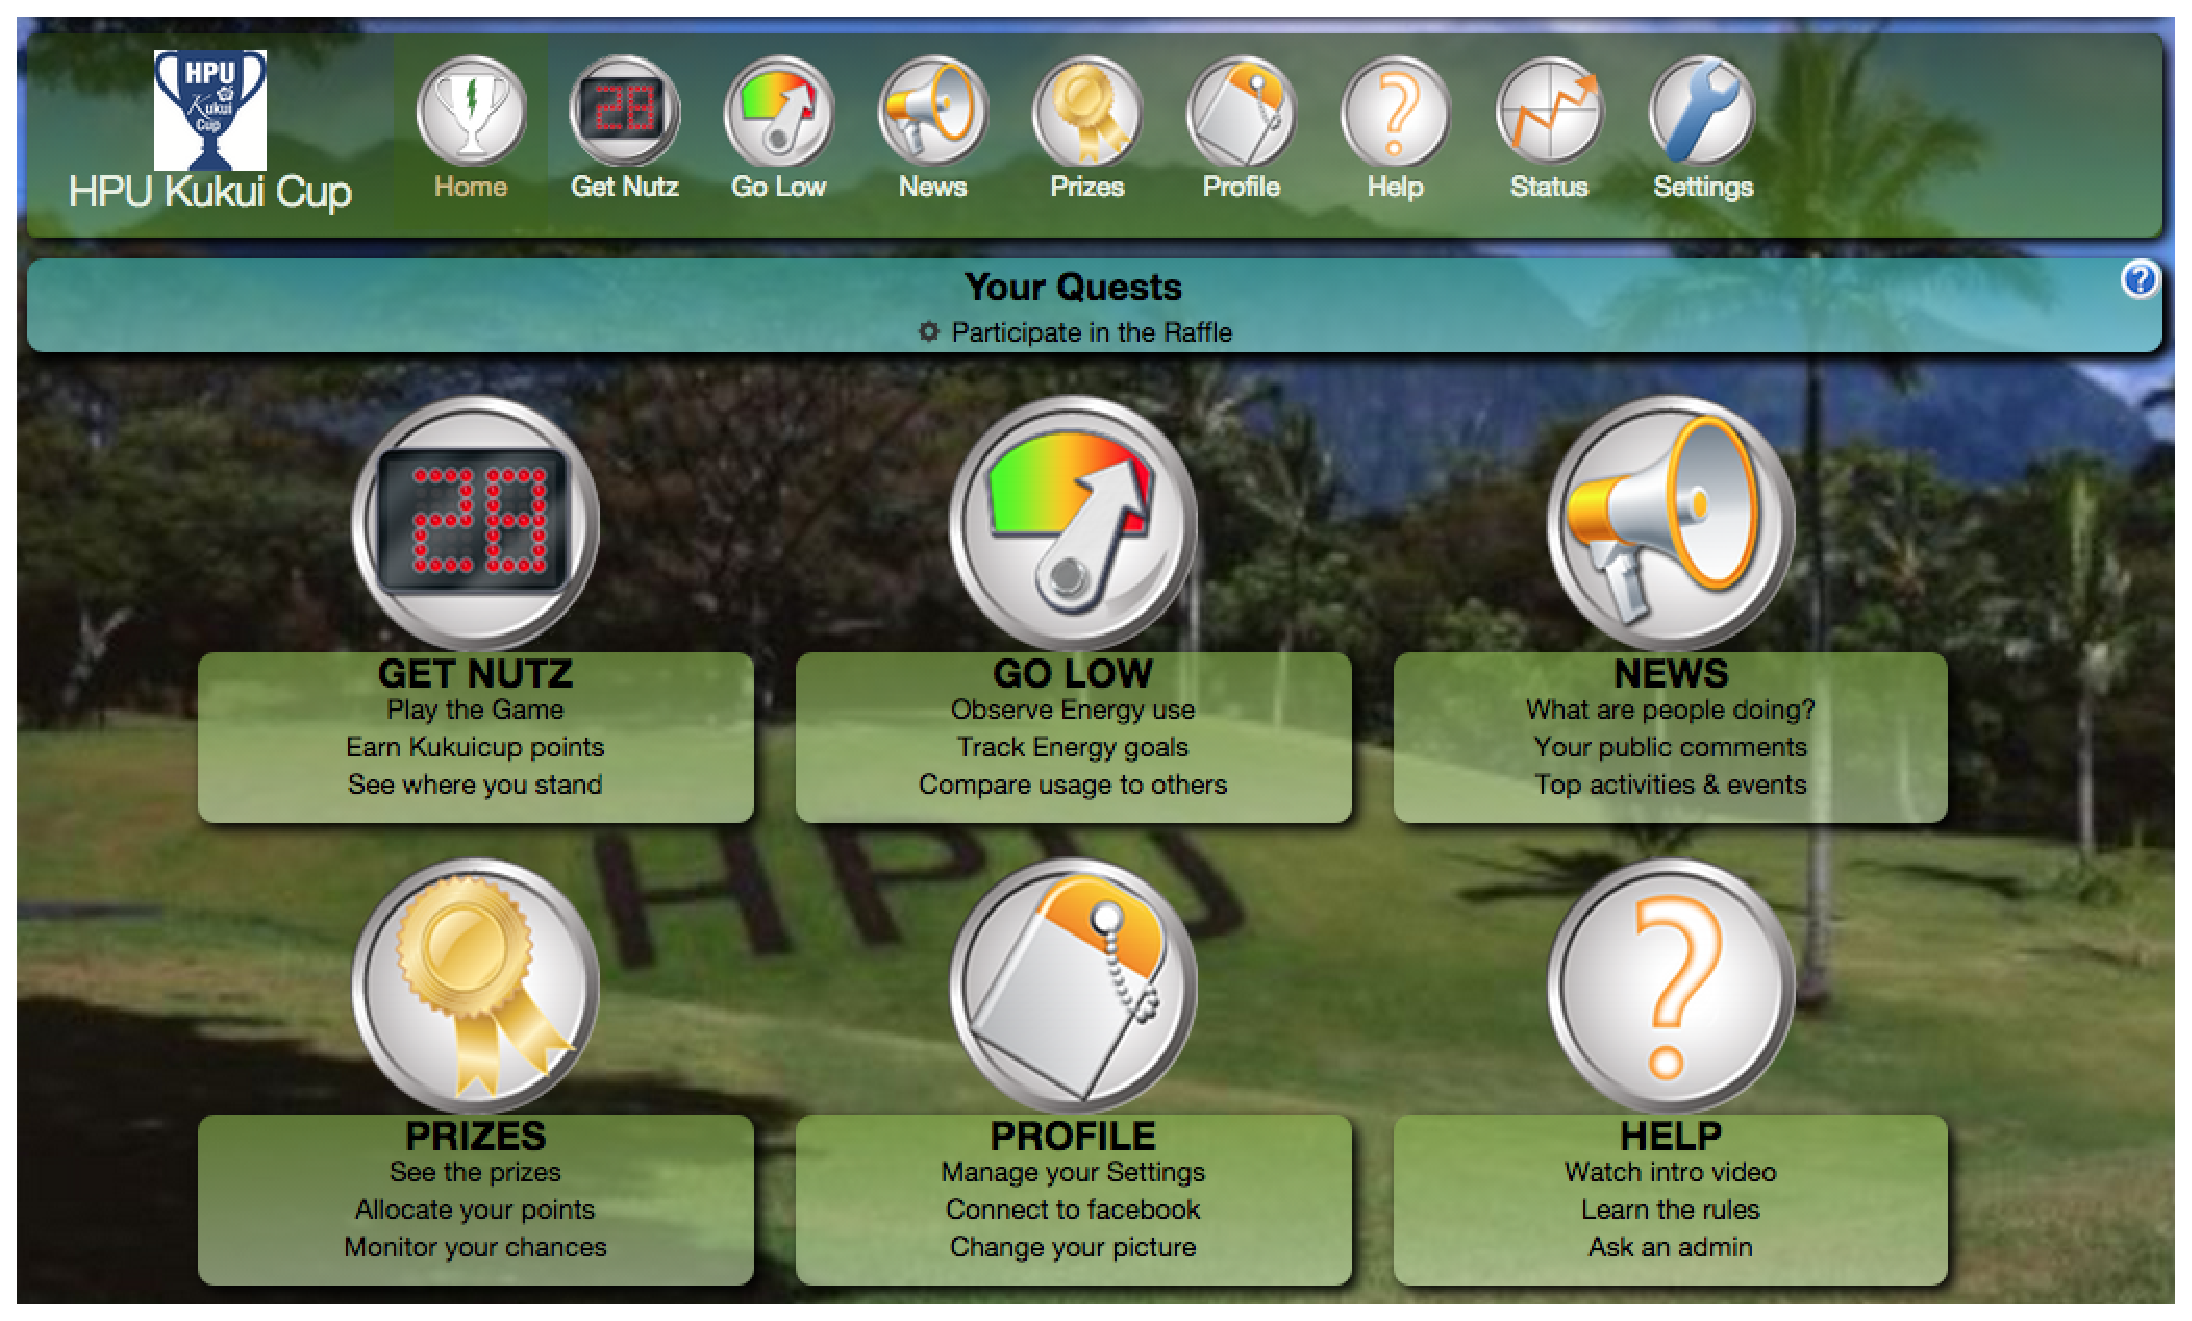
\includegraphics[width=20em]{hpu-homepage}
   \caption{HPU Kukui Cup Challenge Home Page}
   \label{fig:hpu-homepage}
\end{figure}

\subsection{East-West Center}

The EWC Kukui Cup Energy and Water challenge was implemented by an international organization called the East-West Center (EWC) using the Makahiki framework. It was held in 2013 for approximately 600 international students living in their residence halls in Hawaii. The challenge lasts for 2 weeks and includes energy and water saving competition between two residence halls. The residence halls did not have internet-enabled smart meters.

\begin{figure}[ht!]
   \centering
   \includegraphics[width=20em]{ewc-homepage}
   \caption{EWC Kukui Cup Challenge Home Page}
   \label{fig:ewc-homepage}
\end{figure}

\subsection{Holy Nativity School}

A pilot instance of Kukui Cup challenge implemented by using the Makahiki framework was held at the Holy Nativity School (HNS), a private elementary school in Hawaii, in 2013. The pilot instance was organized by the school with the partnership with Project Learning Tree (PLT) GreenSchool! program\cite{plt-greenschools}. The nationwide environmental service-learning program helps improve students’ academic performance in STEM subjects by engaging students in STEM as they solve environmental issues at their school.

\begin{figure}[ht!]
   \centering
   \includegraphics[width=20em]{hns-homepage}
   \caption{HNS Kukui Cup Challenge Home Page}
   \label{fig:hns-homepage}
\end{figure}

\subsection{Customization of the Makahiki Instances}

The following sections describe the different customizations that were done to the above Makahiki instances according to the different organizations' needs.

\subsubsection{Configuration Customization}
The challenge configuration includes the duration of the challenge, the participant accounts, resource such as energy and water settings, learning action configurations, prize and other game mechanics settings. 

Table \autoref{table:challenge-configurations} lists the different configurations between the seven real world instances of Makahiki.

\begin{table}[ht!]
  \centering
  \begin{tabular} {|c|c|c|c|c|c|c|c|c|}
    \hline
    \tabhead{Instances} &
    \tabhead{Participants} &
    \tabhead{Teams} &
    \tabhead{Duration} &
    \tabhead{Rounds} &
    \tabhead{Energy Game} &
    \tabhead{Water Game} &
    \tabhead{Prize Game} &
    \tabhead{Quest Game} \\
    \hline
    UHM2011 & 1000 & 20 & 3 weeks & 3 & Yes & No & Yes & Yes\\
    \hline
    UHM2012 & 1086 & 20 & 9 months & 3 & Yes & No & Yes & Yes\\
    \hline
    UHM2014 & 1093 & 20 & 2 weeks & 3 & Yes & No & Yes & Yes\\
    \hline
    HPU2012 & 190 & 6 & 3 weeks & 3 & Yes & No & Yes & Yes\\
    \hline
    HPU2013 & 190 & 6 & 3 weeks & 3 & Yes & No & Yes & Yes\\
    \hline
    EWC2012 & 130 & 2 & 2 weeks & 3 & Yes  & Yes & No & No\\
    \hline
    HNS2013 & 10 & 2 & 4 weeks & 3 & No & No & Yes & Yes \\
    \hline
  \end{tabular}
  \caption{Challenge Configuration Differences}
  \label{table:challenge-configurations}
\end{table}

As we can see from the Table \autoref{table:challenge-configurations}, the Makahiki framework can be customized to support different size of the team competition with different duration, with energy, water and both competition, as well as the different education contents of
the sponsoring organizations. For example, while UHM and HPU
challenges involved only energy consumption data, the EWC challenge involved both energy
and water consumption data. 

\subsubsection{Content Customization}
Because the different organizations have different sustainability educational needs, they used the Makahiki framework to customize the content, which is shown to student players via the SmartGrid Game mechanics. They can re-use or modify the existing contents came with the Makahiki framework or create new content to be included in the system. The table \autoref{table:sgg-configuration} shows the difference in the type and layout of the educational contents. UHM had the most number of the learning actions while HNS has the least. 

\begin{table}[ht!]
  \centering
  \begin{tabular} {|c|c|c|c|c|c|c|}
    \hline
    \tabhead{Instances} &
    \tabhead{Levels} &
    \tabhead{Activities} &
    \tabhead{Commitments} &
    \tabhead{Events} & 
    \tabhead{Total Actions}\\
    \hline
    UHM2011 & 1 & 40 & 1 & 40  & 499\\
    \hline
    UHM2012 & 7 & 60 & 1 & 40  & 499 \\
    \hline
    UHM2014 & 4 & 34 & 1 & 40  & 499\\
    \hline
    HPU2012 & 3 & 22 & 1 & 40  & 499 \\
    \hline
    HPU2013 & 3 & 33 & 1 & 40  & 499 \\
    \hline
    EWC2012 & 4 & 11 & 1 & 40  & 499 \\
    \hline
    HNS2013 & 2 & 22 & 1 & 40  & 499 \\
    \hline
  \end{tabular}
  \caption{Content Differences}
  \label{table:sgg-configurations}
\end{table}

The layout of the educational content represented in the SmartGrid game is also highly customizable to include different levels, rows and columns. The figures  \autoref{fig:UH-SGG}, \autoref{fig:HPU-SGG}, \autoref{fig:EWC-SGG}, \autoref{fig:GS-SGG} illustrate the content and layout of the educational SmartGrid game in the different Makahiki instances. 

\begin{figure}[http]
	\centering
		\subfigure[UHM 2011 Kukui Cup SmartGrid Game]{\label{fig:uh-2011}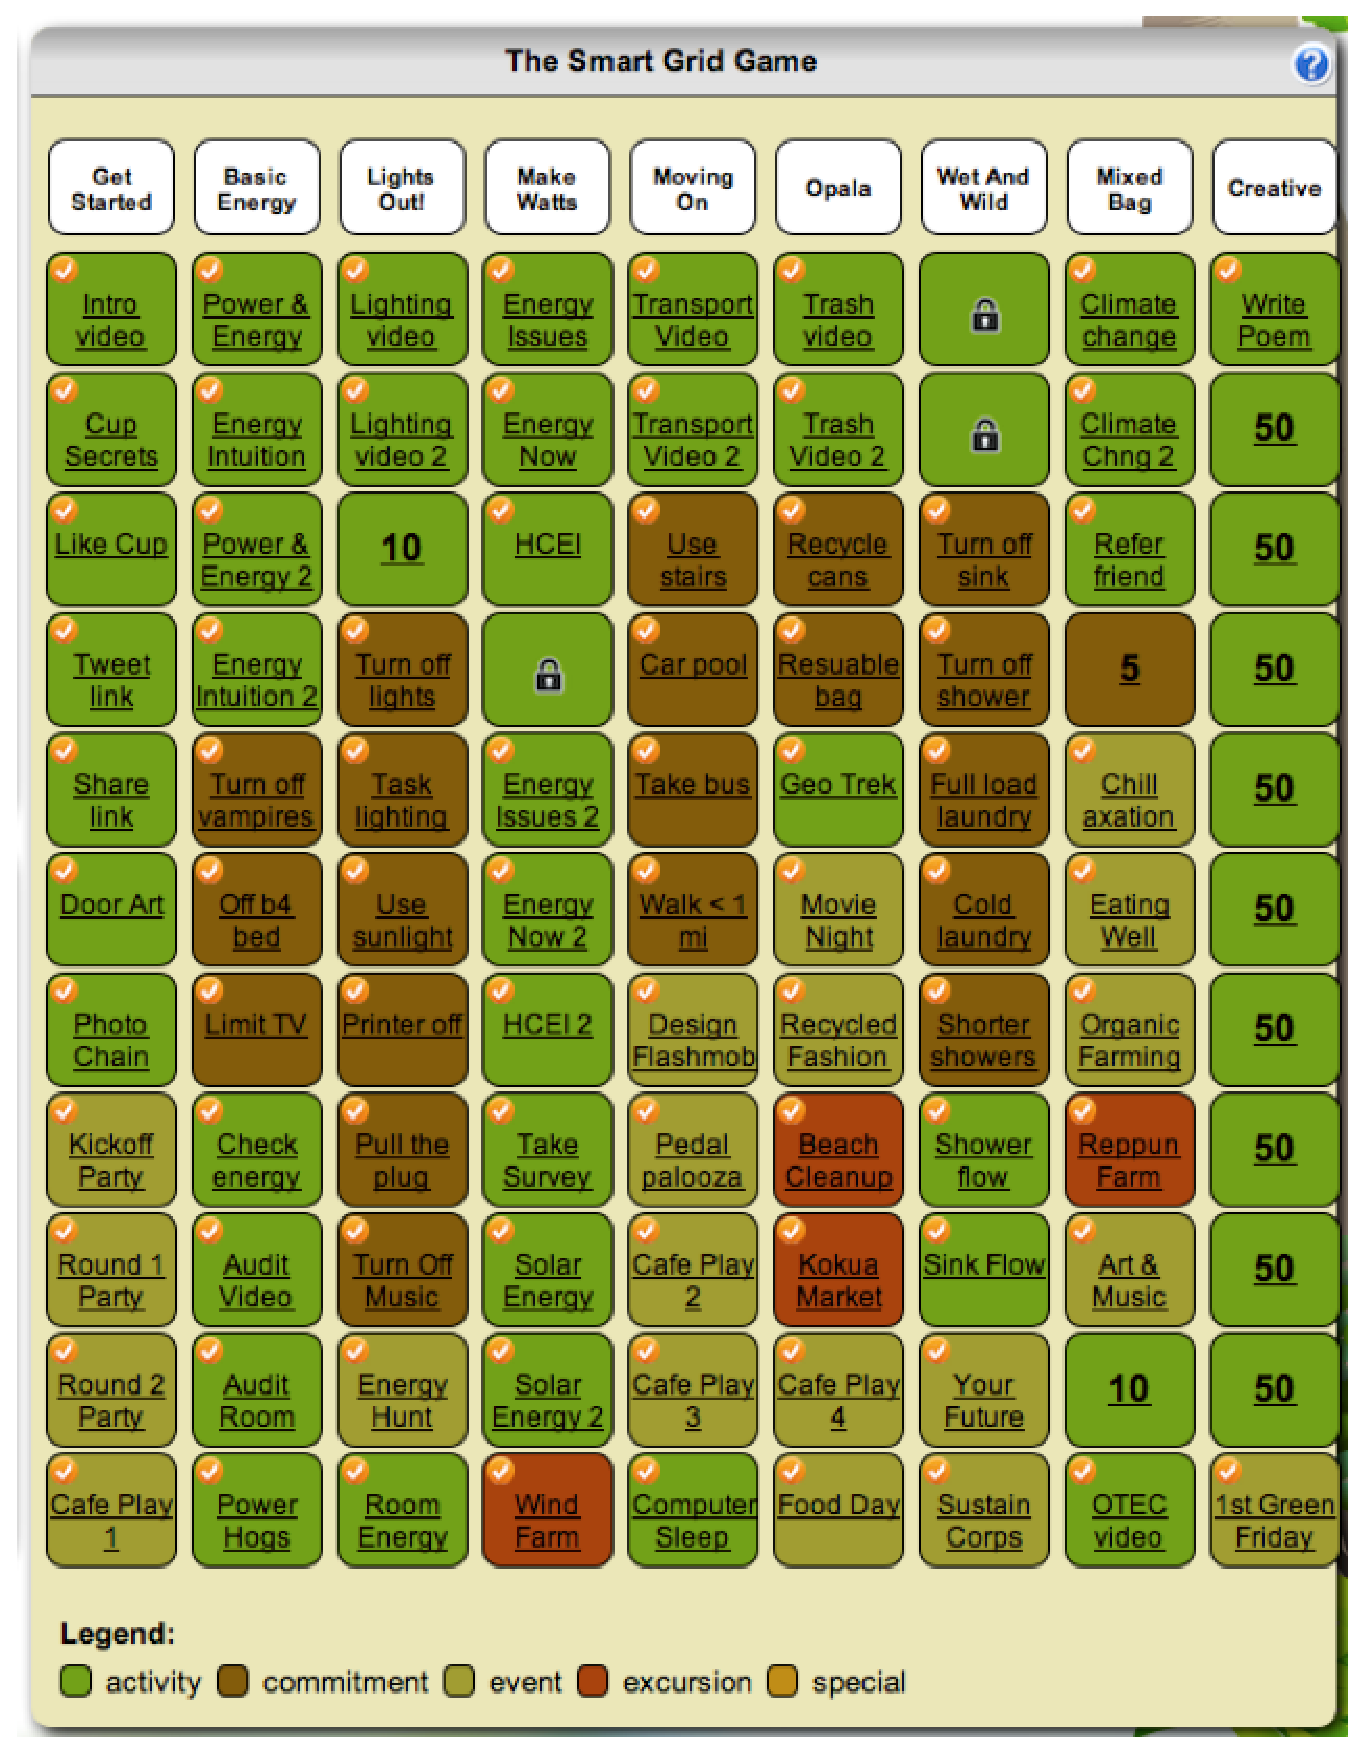
\includegraphics[height=4in,width=3.5in]{UH-SGG-2011.eps}}
		\subfigure[UHM 2012 Kukui Cup SmartGrid Game]{\label{fig:uh-2012}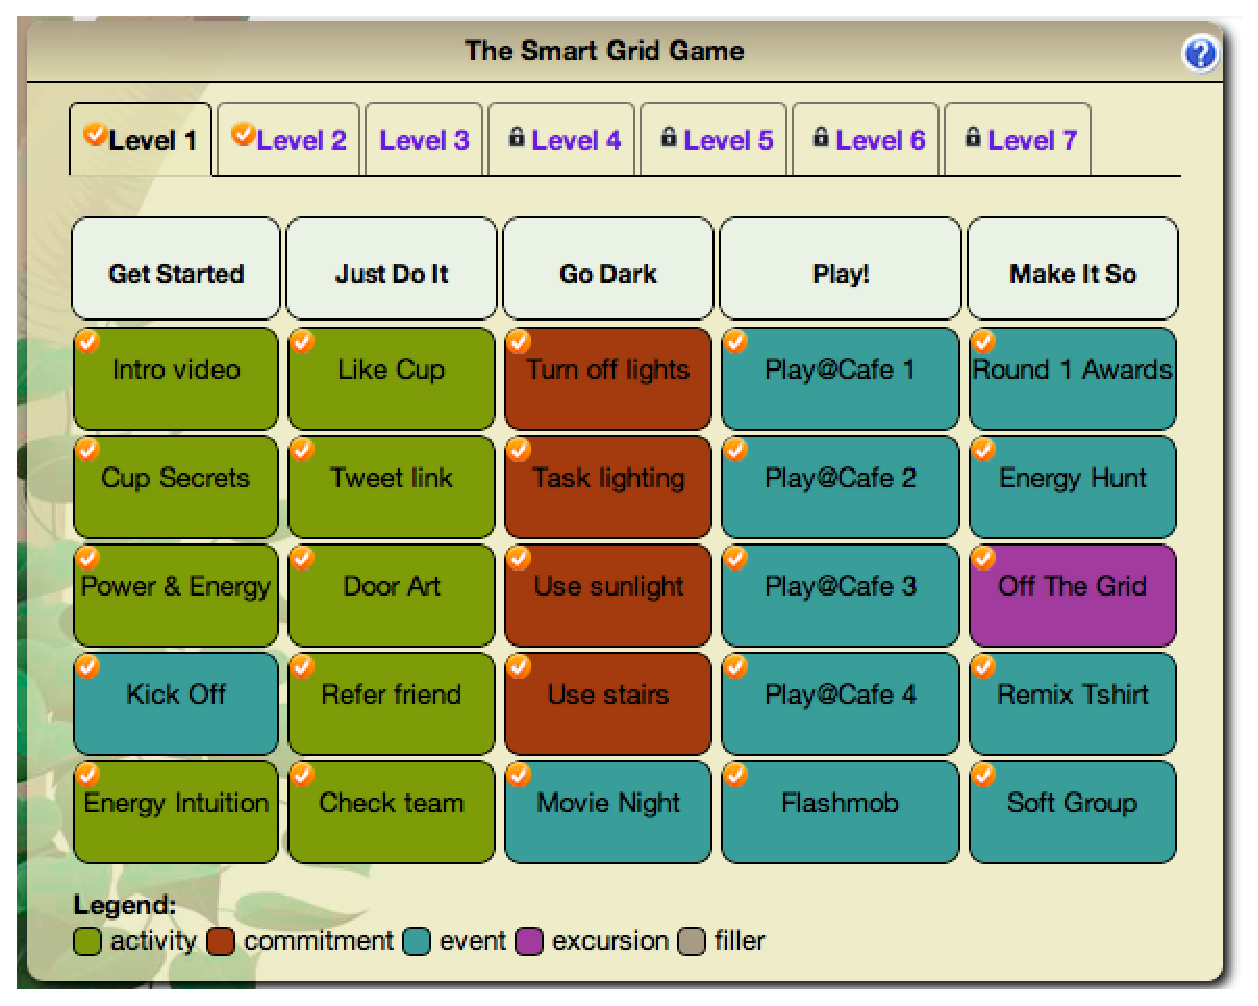
\includegraphics[height=2.3in,width=3.5in]{UH-SGG-2012.eps}}
		\subfigure[UHM 2014 Kukui Cup SmartGrid Game]{\label{fig:uh-2014}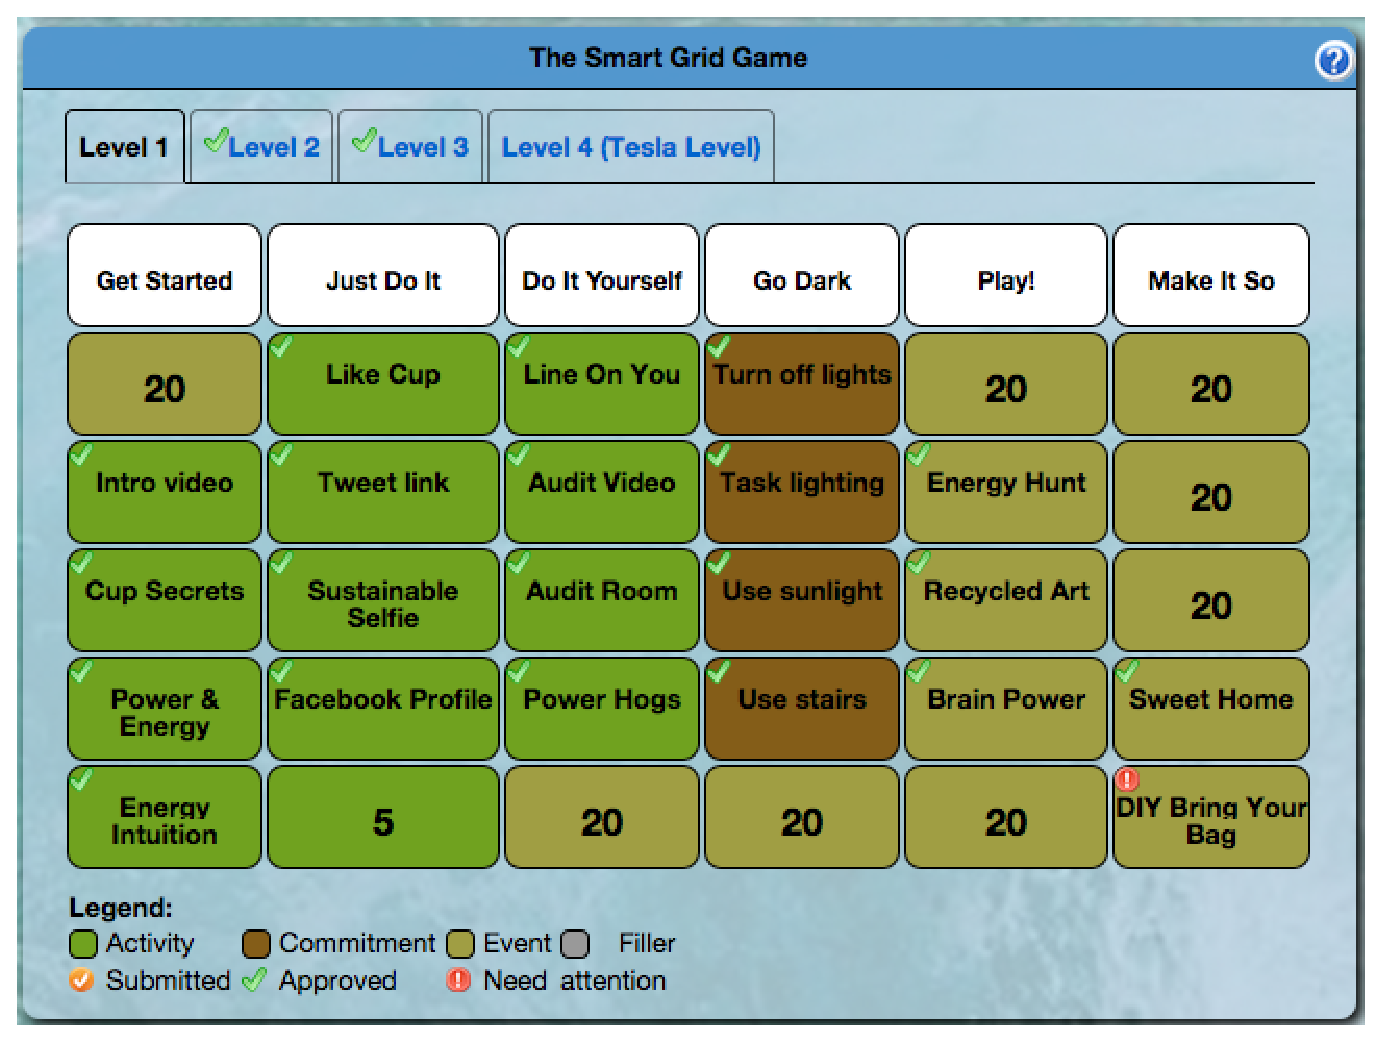
\includegraphics[height=2.3in,width=3.5in]{UH-SGG-2014.eps}}
		\caption{UHM SmartGrid Game Layouts}
		\label{fig:UHM-SGG}
\end{figure}

\begin{figure}[htbp]
	\centering
		\subfigure[HPU SmartGrid Game Level1]{\label{fig:hpu-level1}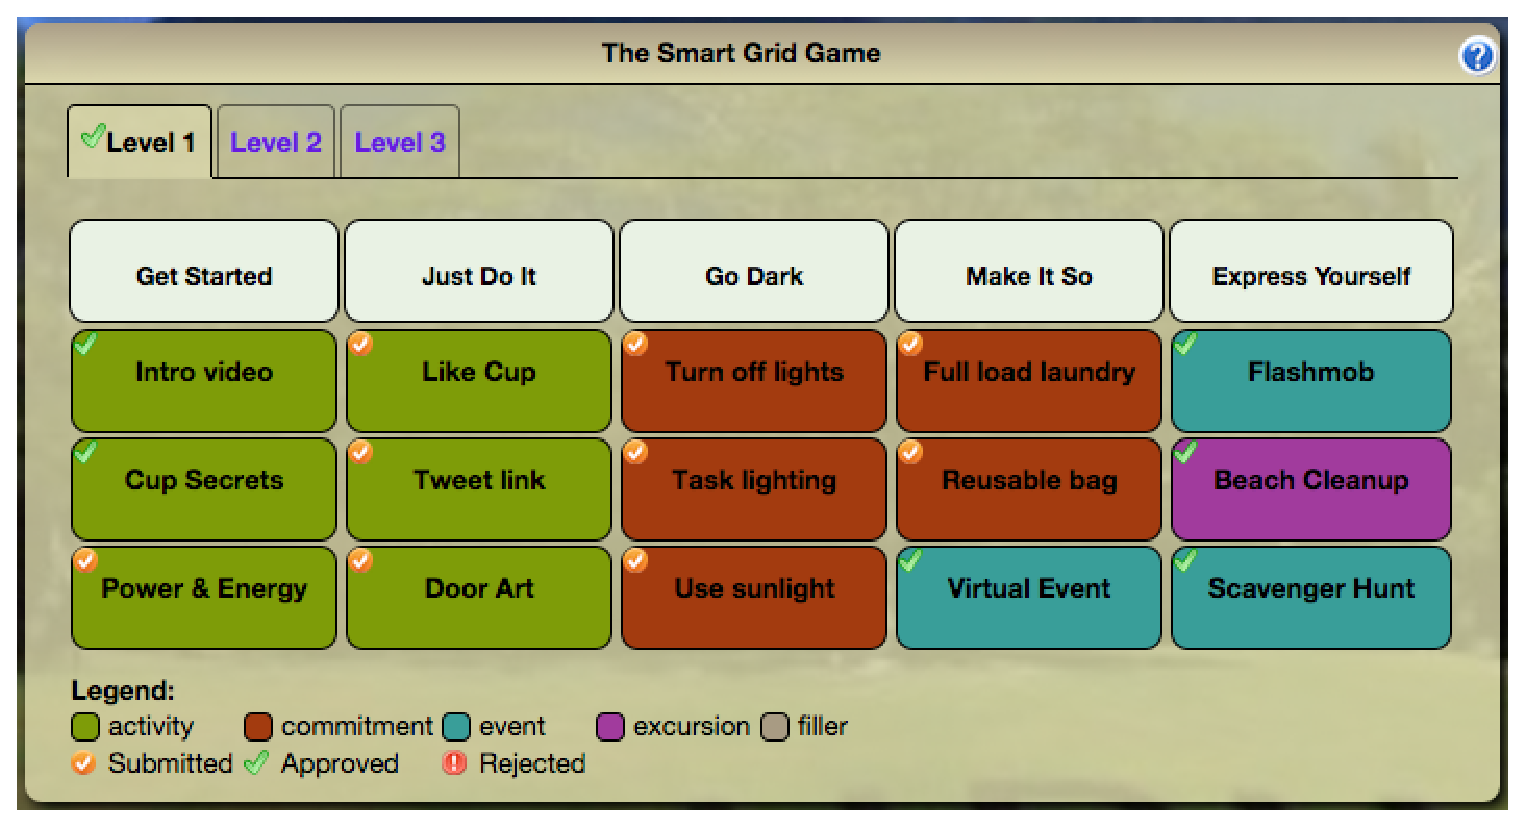
\includegraphics[height=2in,width=3.5in]{HPU-SGG-level1.eps}}
		\subfigure[HPU SmartGrid Game Level2]{\label{fig:hpu-level2}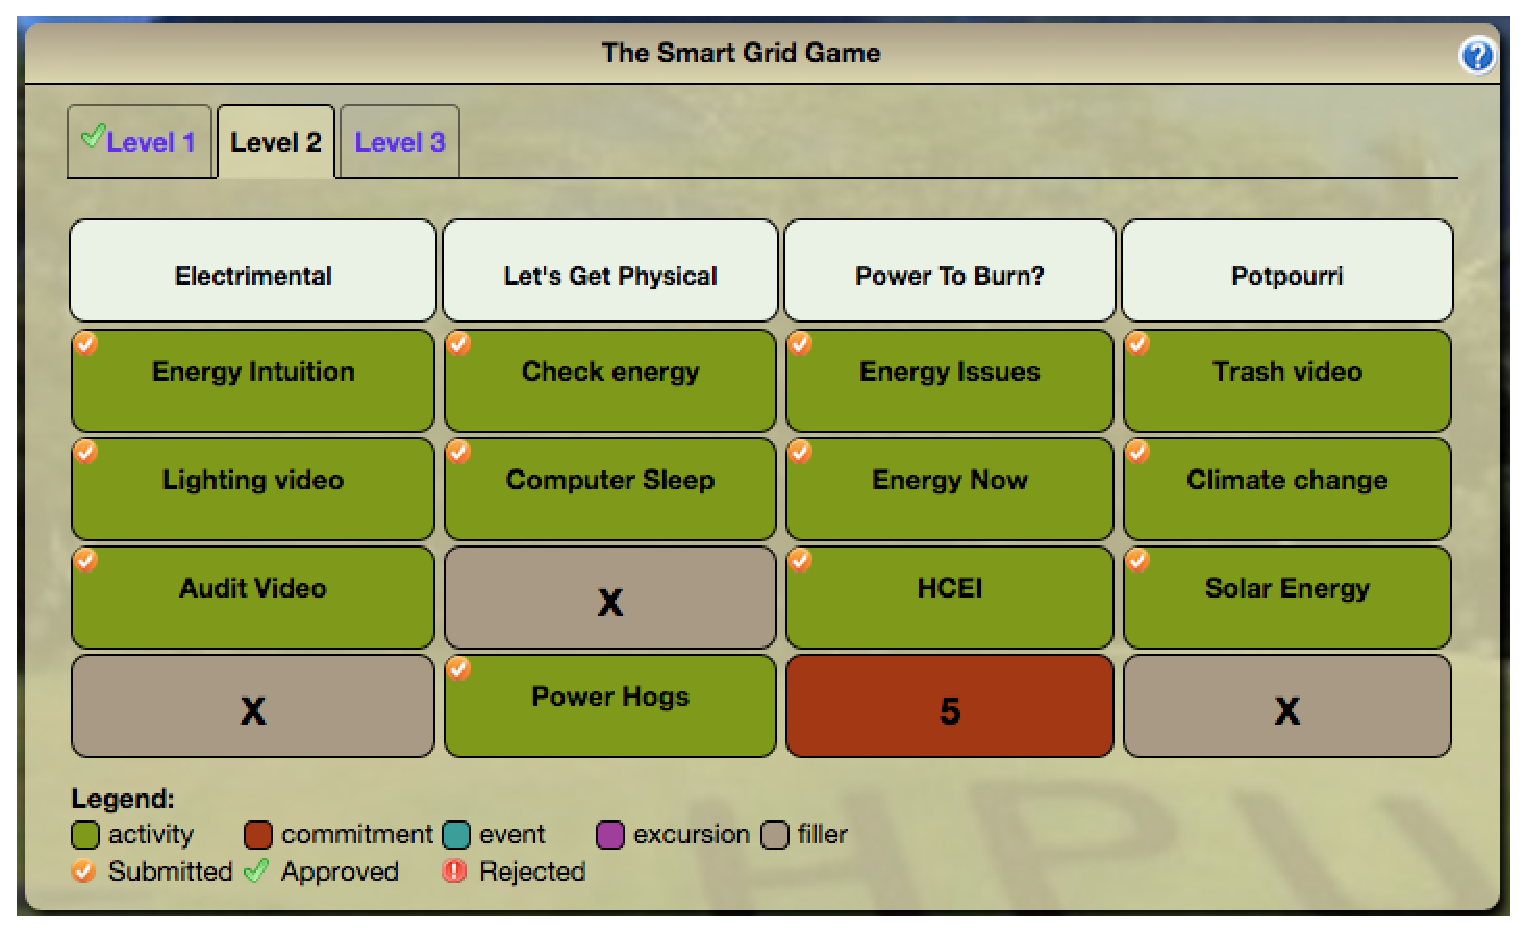
\includegraphics[height=2in,width=3.5in]{HPU-SGG-level2.eps}}
		\subfigure[HPU SmartGrid Game Level3]{\label{fig:hpu-level3}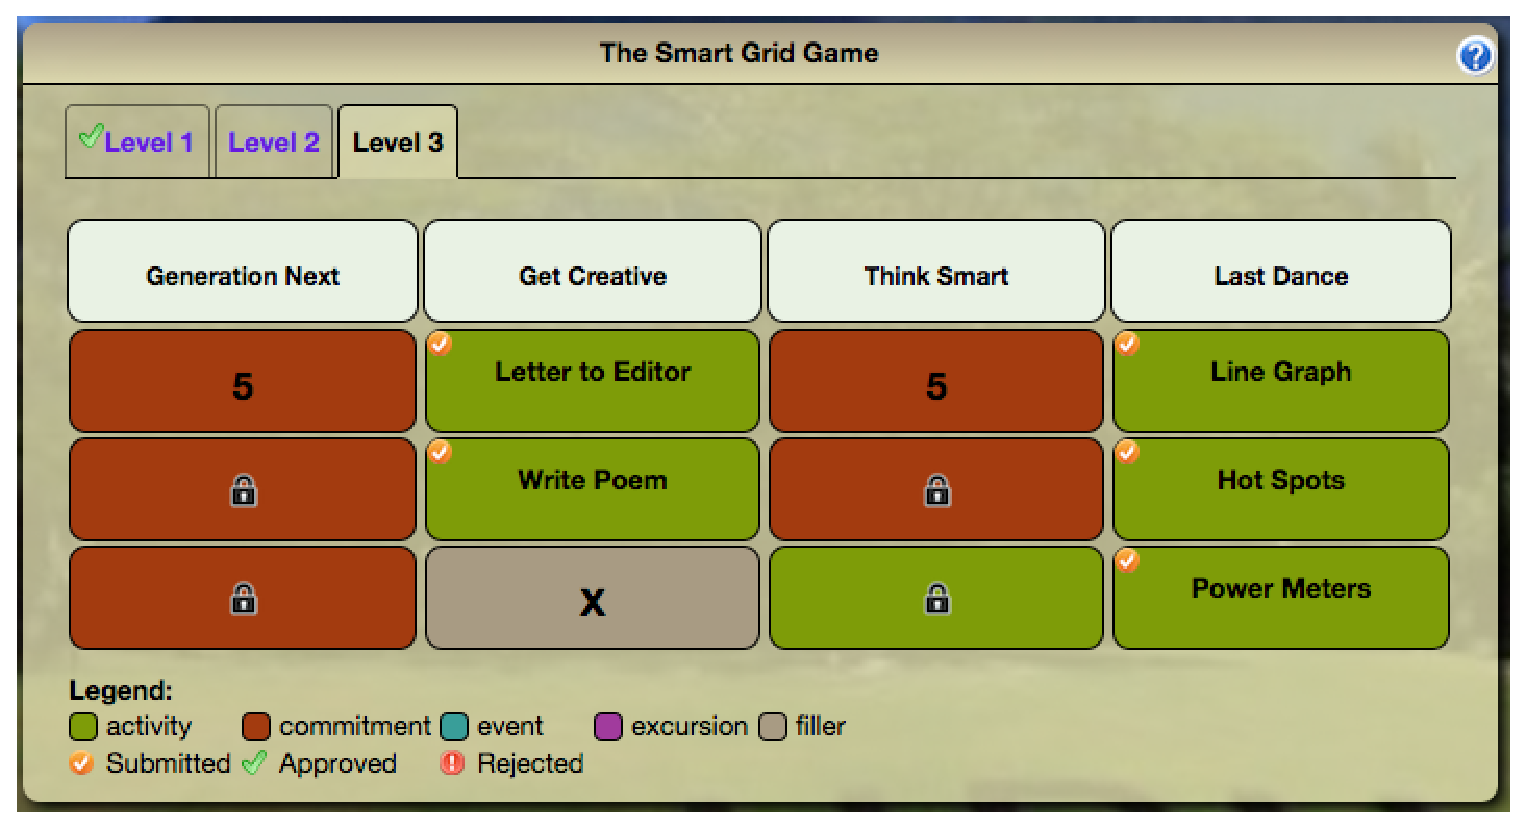
\includegraphics[height=2in,width=3.5in]{HPU-SGG-level3.eps}}
		\caption{HPU SmartGrid Game Layouts}
		\label{fig:HPU-SGG}
\end{figure}

\begin{figure}[htbp]
	\centering
		\subfigure[EWC SmartGrid Game Level1]{\label{fig:ewc-level1}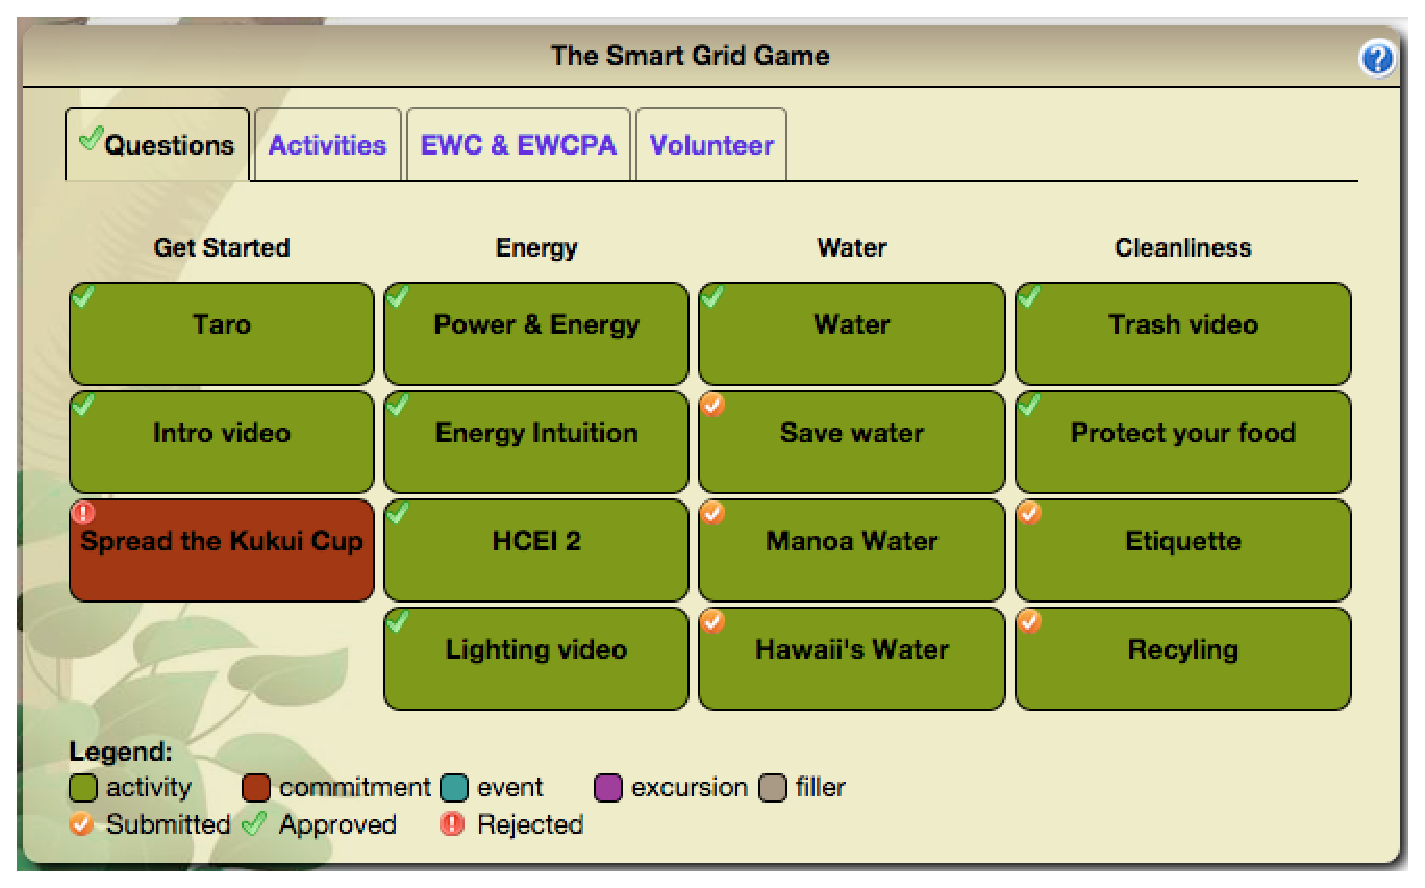
\includegraphics[height=2in,width=3.5in]{EWC-SGG-level1.eps}}
		\subfigure[EWC SmartGrid Game Level2]{\label{fig:ewc-level2}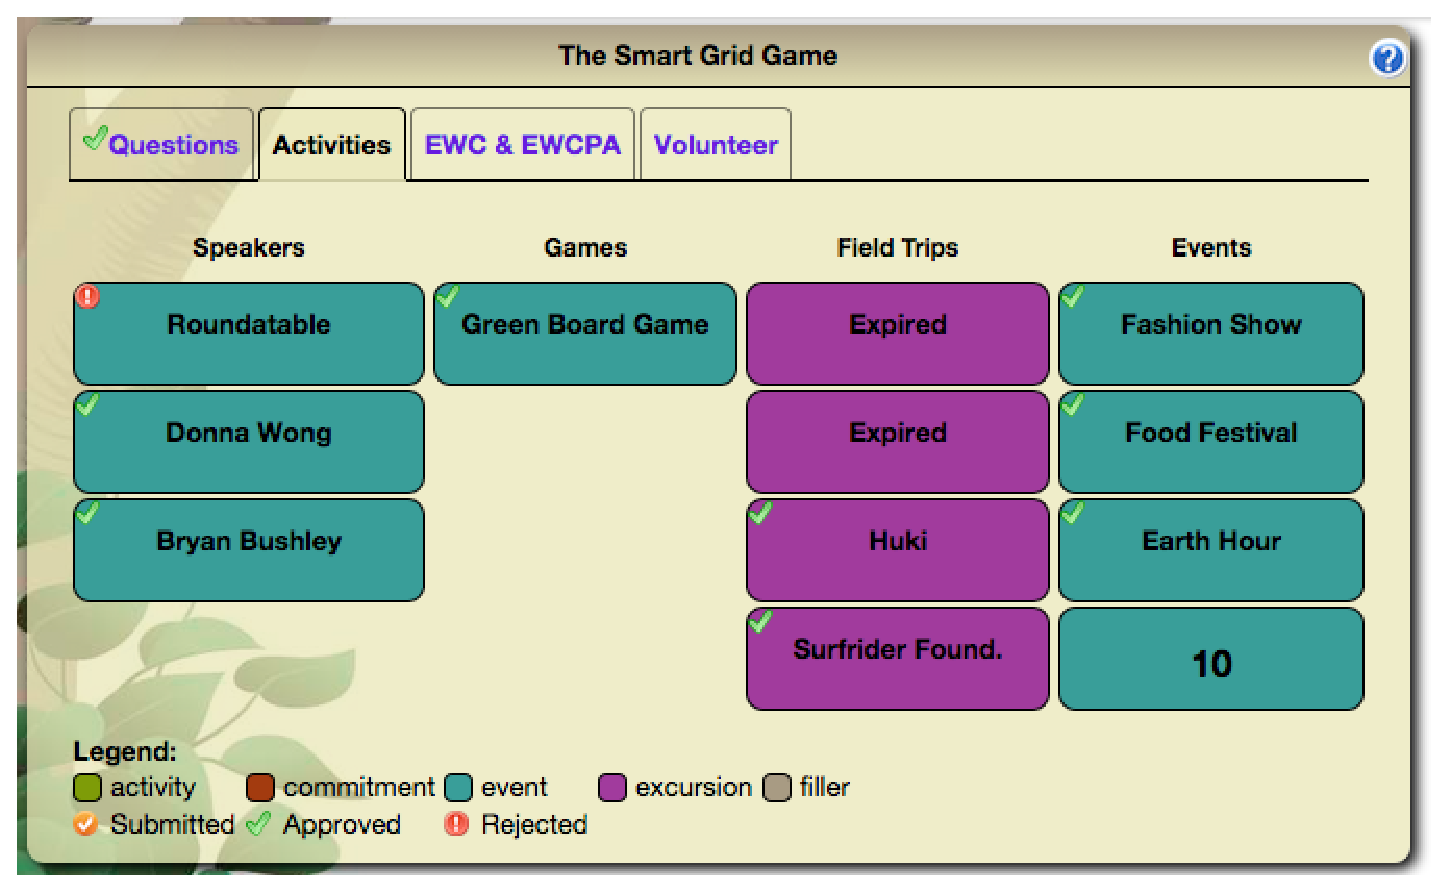
\includegraphics[height=2in,width=3.5in]{EWC-SGG-level2.eps}}
		\subfigure[EWC SmartGrid Game Level3]{\label{fig:ewc-level3}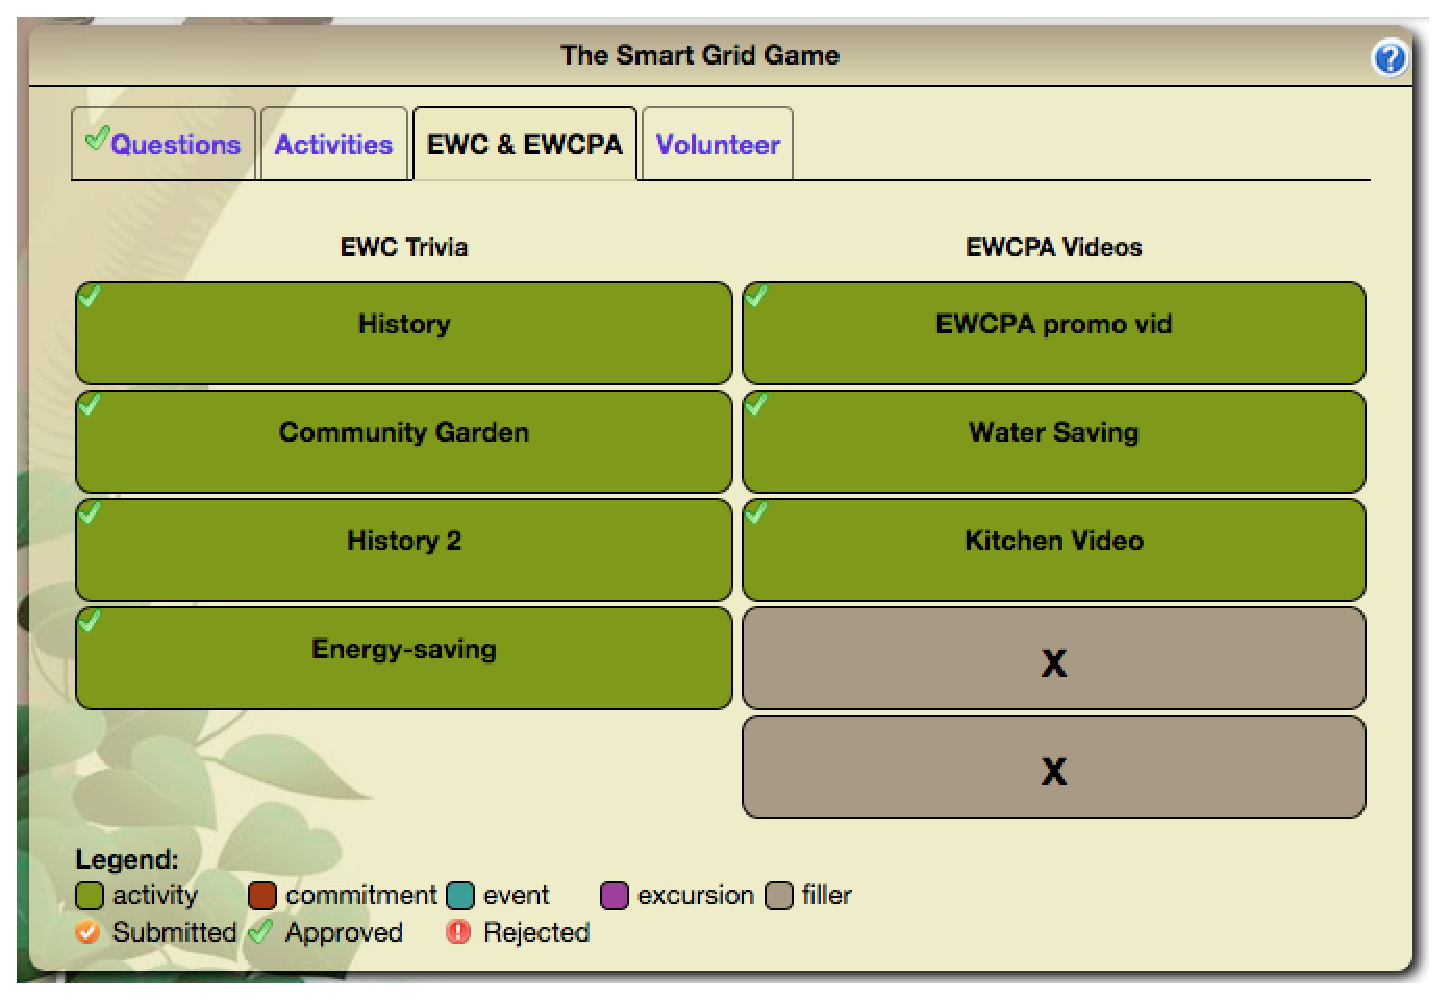
\includegraphics[height=2in,width=3.5in]{EWC-SGG-level3.eps}}
		\subfigure[EWC SmartGrid Game Level4]{\label{fig:ewc-level4}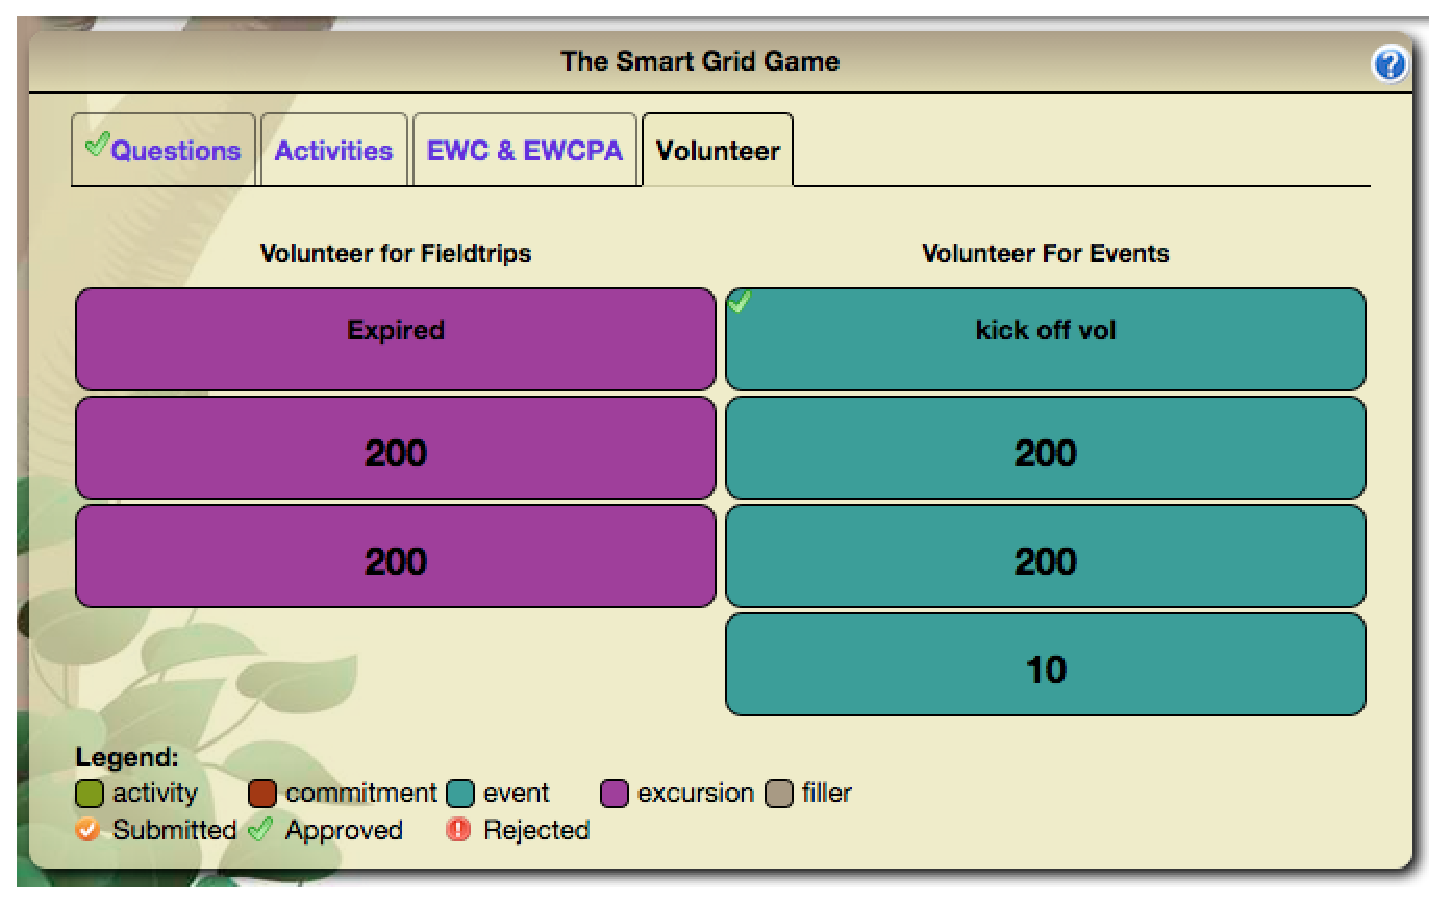
\includegraphics[height=2in,width=3.5in]{EWC-SGG-level4.eps}}
		\caption{EWC SmartGrid Game Layouts}
		\label{fig:EWC-SGG}
\end{figure}

\begin{figure}[htbp]
	\centering
		\subfigure[HNS SmartGrid Game Level1]{\label{fig:gs-level1}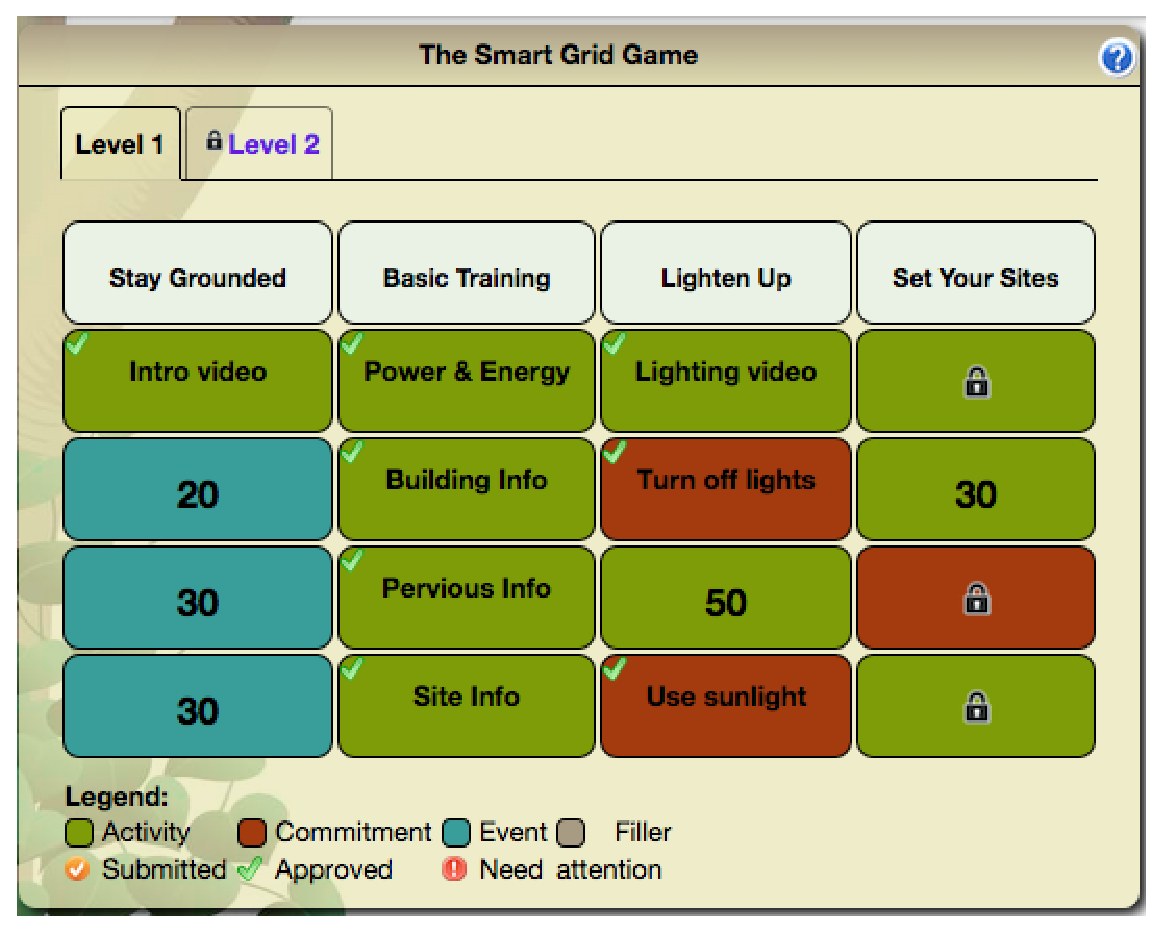
\includegraphics[height=2in,width=3.5in]{GS-SGG-level1.eps}}
		\subfigure[HNS SmartGrid Game Level2]{\label{fig:gs-level2}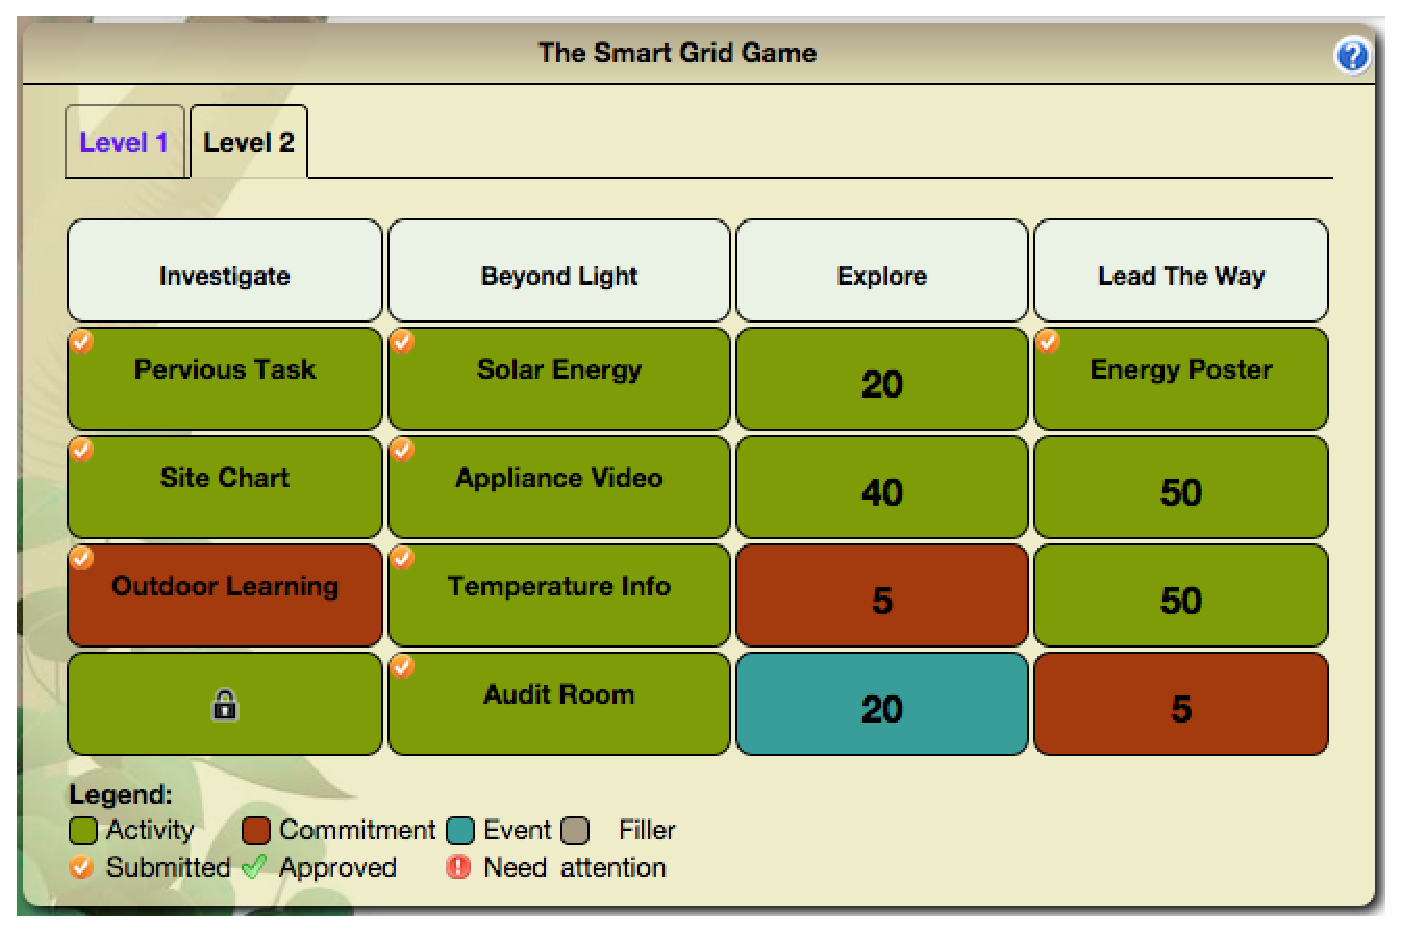
\includegraphics[height=2in,width=3.5in]{GS-SGG-level2.eps}}
		\caption{HNS SmartGrid Game Layouts}
		\label{fig:GS-SGG}
\end{figure}

\subsubsection{Branding Customization}
The look and feel of the challenges website are difference between the different organizations, which is customized using the customization feature of the Makahiki framework. The user interface was customized to ``brand'' each challenge. The list of customizable branding are:

\begin{itemize}
\item logo
\item size name
\item challenge name
\item team label
\item landing page text
\item about page text
\item sponsor text and logo
\item theme
\end{itemize}

\subsubsection{System Configuration}

The system configuration includes the infrastructure hosting, user authentication, and smart meter connections. 

Table \autoref{table:system-configurations} lists the different configurations between the seven real world instances of Makahiki.

\begin{table}[ht!]
  \centering
  \begin{tabular} {|c|c|c|c|c|c|c|}
    \hline
    \tabhead{Instances} &
    \tabhead{Hosting} &
    \tabhead{Authentication} &
    \tabhead{Smart meters} \\
    \hline
    UHM2011 & Local & CAS & Yes \\
    \hline
    UHM2012 & Cloud & CAS & Yes \\
    \hline
    UHM2014 & Cloud & CAS & Yes \\
    \hline
    HPU2012 & Local & LDAP & Yes \\
    \hline
    HPU2013 & Local & LDAP & Yes \\
    \hline
    EWC2012 & Cloud & CAS \& Internal & No \\
    \hline
    HNS2013 & Cloud & Internal & No \\
    \hline
  \end{tabular}
  \caption{System Configuration Differences}
  \label{table:system-configurations}
\end{table}
 
UH and HPU used different metering infrastructure, and EWC collected their resource data manually.  Since the
halls did not have internet-enabled meters, resource consumption data had to be entered by
the game managers manually.

The IT infrastructure at UH and HPU provided
authentication services using CAS (Central Authentication Service) and LDAP, while EWC
used the built-in Django authentication.  

\section{SGSEAM assessment}

The successful creation of serious game challenges by four different organizations
provides evidence that Makahiki can be successfully tailored to the needs of different organizations. This section describes the result of applying a formal assessment method of SGSEAM to the Makahiki framework to assess the strengths and weaknesses of the Makahiki as a serious game framework.

The table \autoref{fig:assessment-overview} provides the overview of applying SGSEAM to Makahiki.

\begin{figure}[ht!]
  \centering
  \begin{tabular}{|c|c|c|}
    \hline
    \multicolumn{1}{|p{0.2\columnwidth}|}{\centering\tabhead{Stakeholder}} &
    \multicolumn{1}{|p{0.5\columnwidth}|}{\centering\tabhead{Assessment Approach}} &
    \multicolumn{1}{|p{0.2\columnwidth}|}{\centering\tabhead{Experiements}}  \\
    \hline
    \multicolumn{1}{|p{0.2\columnwidth}|}{\multirow{4}{*}{Players}} &
    \multicolumn{1}{|p{0.5\columnwidth}|}{Pre Post effectiveness study} &
    \multicolumn{1}{|p{0.2\columnwidth}|}{UHM KC} \\
    \cline{2-3}
    \multicolumn{1}{|p{0.2\columnwidth}|}{} &
    \multicolumn{1}{|p{0.5\columnwidth}|}{Self-reported effectiveness survey} &
    \multicolumn{1}{|p{0.2\columnwidth}|}{UHM KC} \\
    \cline{2-3}    
    \multicolumn{1}{|p{0.2\columnwidth}|}{} &
    \multicolumn{1}{|p{0.5\columnwidth}|}{Self-reported usability survey} &
    \multicolumn{1}{|p{0.2\columnwidth}|}{UHM KC} \\
    \cline{2-3}
    \multicolumn{1}{|p{0.2\columnwidth}|}{} &
    \multicolumn{1}{|p{0.5\columnwidth}|}{Engagement metrics} &
    \multicolumn{1}{|p{0.2\columnwidth}|}{UHM KC} \\
    \hline
    \multicolumn{1}{|p{0.2\columnwidth}|}{\multirow{2}{*}{System admins}} &
    \multicolumn{1}{|p{0.5\columnwidth}|}{In-lab installation study} &
    \multicolumn{1}{|p{0.2\columnwidth}|}{ICS691} \\
    \cline{2-3}
    \multicolumn{1}{|p{0.2\columnwidth}|}{} &
    \multicolumn{1}{|p{0.5\columnwidth}|}{Post-hoc system admin interview} &
    \multicolumn{1}{|p{0.2\columnwidth}|}{HPU KC} \\
    \hline
    \multicolumn{1}{|p{0.2\columnwidth}|}{\multirow{2}{*}{Game designers}} &
    \multicolumn{1}{|p{0.5\columnwidth}|}{In-lab game design study} &
    \multicolumn{1}{|p{0.2\columnwidth}|}{ICS691} \\
    \cline{2-3}
    \multicolumn{1}{|p{0.2\columnwidth}|}{} &
    \multicolumn{1}{|p{0.5\columnwidth}|}{Post-hoc game designer interview} &
    \multicolumn{1}{|p{0.2\columnwidth}|}{HPU KC} \\
    \hline
    \multicolumn{1}{|p{0.2\columnwidth}|}{\multirow{2}{*}{Game managers}} &
    \multicolumn{1}{|p{0.5\columnwidth}|}{In-lab game management study} &
    \multicolumn{1}{|p{0.2\columnwidth}|}{ICS691} \\
    \cline{2-3}
    \multicolumn{1}{|p{0.2\columnwidth}|}{} &
    \multicolumn{1}{|p{0.5\columnwidth}|}{Post-hoc game manager interview} &
    \multicolumn{1}{|p{0.2\columnwidth}|}{HPU KC} \\
    \hline
    \multicolumn{1}{|p{0.2\columnwidth}|}{Developers} &
    \multicolumn{1}{|p{0.5\columnwidth}|}{In-lab game development study} &
    \multicolumn{1}{|p{0.2\columnwidth}|}{ICS691} \\
    \hline
  \end{tabular}
  \caption{SGSEAM assessments for Makahiki}
  \label{fig:assessment-overview}
\end{figure}

\subsection{Makahiki Player Assessment}

We used four approaches to assess the player experience for the Makahiki framework. They are pre-post effectiveness study, self-report effectiveness survey, self-report usability survey, and engagement metrics. The real world Makahiki instances of UHM Kukui Cup challenge were used for the Makahiki player assessments. 

\subsubsection{Pre Post effectiveness study}

In the 2011 Kukui Cup Challenge at the University of Hawaii at Manoa, a serious game implemented using the Makahiki framework, there were over 1000 eligible players for this challenge, who were mostly first
year college students living in the 5 resident halls. The challenge was designed to lasted for 3 weeks and the student players are divided into 20 teams based on the dorm locations where they resided, each team's energy consumption is measured a smart meter installed in the various locations inside the resident hall. Makahiki recorded the energy consumption for the players before, during and after the challenge. Makahiki also recorded detailed logging data from every interaction between the players and the website. 

To assess the effectiveness of the framework for designing games that improve player literacy in sustainability, 
 two energy literacy surveys were conducted, one before the challenge (pre-game) and one after
the challenge (post-game). 24 players completed both surveys. Out of the total 19 energy
literacy questions, the average number of questions answered correctly is 7.54 before the
challenge, and 8.96 after the challenge. This result indicates an 18\% improvement on the
energy literacy.  Non-players as a control condition were also surveyed , and found that
their literacy did not change, indicating that the improvement in player literacy was indeed due to the game.

To assess the effectiveness of the framework for designing games that produce positive change in sustainability
behaviors, The energy consumption data that collected before, during and after the
challenge were used to compare the differences.  Before the challenge, an energy usage baseline was established. 
During the challenge, compared to the baseline, 12 out of the total 20 teams reduced their energy
consumption, with the highest reduction of 16.1\%. However, 3 teams actually increased
their energy consumption, with the highest increase of 11.7\%. Overall, the average
reduction of the 20 teams was very low---approximately 2\%.

\subsubsection{Self-reported effectiveness survey}
A survey to gather the opinions of participants regarding the effect of the challenge to their sustainability behavior was included at the last round of the challenge. 
Two survey questions was used to assess the self-reported perception of the players regarding the interests in energy conservation and sustainability prior and after playing the Kukui Cup. 

In the 2011 UHM Kukui Cup challenge, 43 players completed the survey. The responses to the survey are in free text. We analyzed the free text responses and coded them into three categories: ``Yes'', ``No'', and ``Somewhat''. \autoref{table:interests-in-sustainability} lists results of the responses. \autoref{fig:effect-prior-after} illustrates the percentages of self-reported interests in the sustainability prior to the KuKui Cup and the effect after playing the Kukui Cup.

\begin{table}[ht!]
  \centering
  \begin{tabular} {|p{0.6\linewidth}|c|c|c|}
    \hline
    \tabhead{\multirow{2}{*}{Question}} & \multicolumn{3}{c|}{\tabhead{Number of Responses}} \\
    \cline{2-4}
    \tabhead{} & \tabhead{Yes} & \tabhead{No } & \tabhead{Somewhat}\\
    \hline
    Prior to playing the Kukui Cup, were you interested in energy conservation? & 24 & 8 & 11\\
    \hline
    Has the Kukui Cup increased your interest in energy conservation and sustainability?& 37 & 0 & 6 \\
    \hline
  \end{tabular}
  \caption{Interests in sustainability prior and after the KC (2011 UHM KC, n=43)}
  \label{table:interests-in-sustainability}
\end{table}

\begin{figure}[htbp]
	\centering
		\subfigure[interests in sustainability prior]{\label{fig:effect-prior}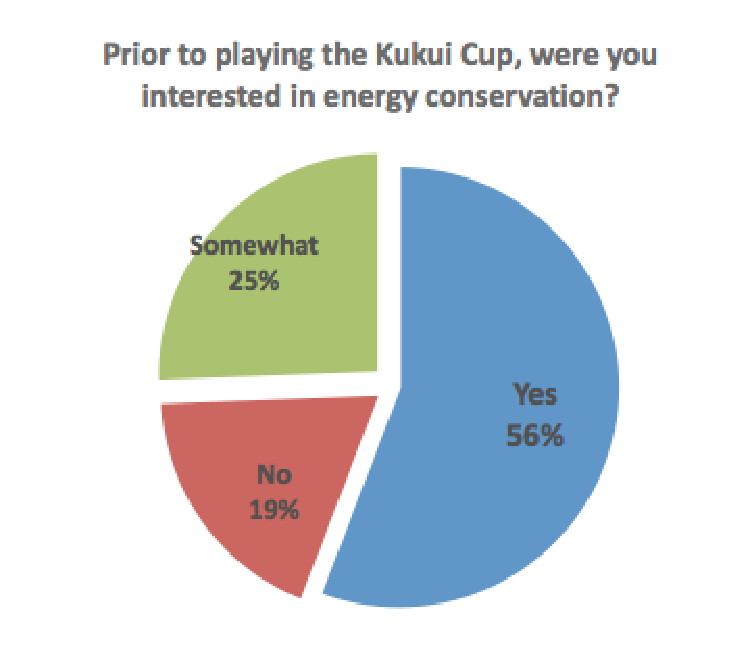
\includegraphics[height=2.2in]{effect-prior.eps}}
		\subfigure[increased interests in sustainability after]{\label{fig:effect-after}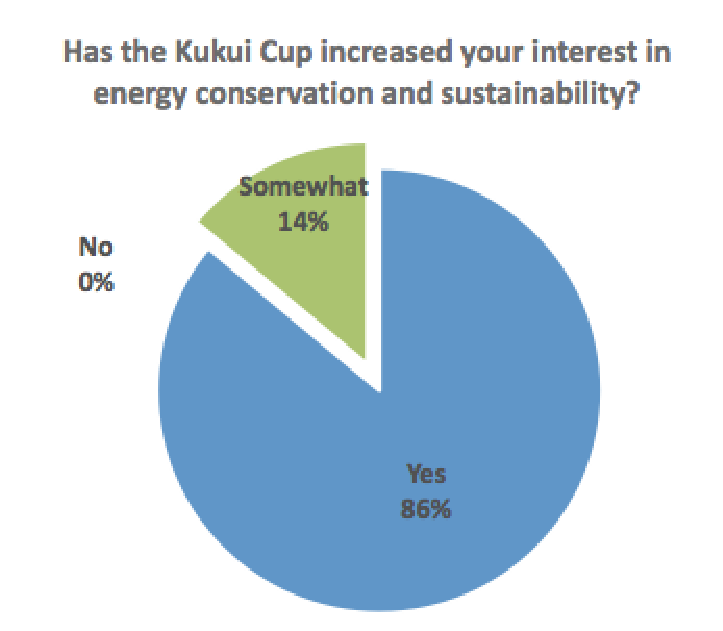
\includegraphics[height=2.2in]{effect-after.eps}}
		\caption{Interests in Sustainability Prior and After the UHM 2011 KC}
		\label{fig:effect-prior-after}
\end{figure}

The self-reported responses indicates that there are a small percentage (19\%) of players were not interested in the sustainability prior to the Kukui Cup. After playing the Kukui Cup, 100\% of responses reported an affirmative or somewhat increase of interests in sustainability. 

In 2012 UHM Kukui Cup challenge, the same survey questions were included the last round. 44 players completed both the two questions. \autoref{table:interests-in-sustainability-2012} lists results of the responses. \autoref{fig:effect-prior-after-2012} illustrates the percentages of self-reported interests.

\begin{table}[ht!]
  \centering
  \begin{tabular} {|p{0.6\linewidth}|c|c|c|}
    \hline
    \tabhead{\multirow{2}{*}{Question}} & \multicolumn{3}{c|}{\tabhead{Number of Responses}} \\
    \cline{2-4}
    \tabhead{} & \tabhead{Yes} & \tabhead{No } & \tabhead{Somewhat}\\
    \hline
    Prior to playing the Kukui Cup, were you interested in energy conservation? & 28 & 4 & 12\\
    \hline
    Has the Kukui Cup increased your interest in energy conservation and sustainability?& 37 & 5 & 2 \\
    \hline
  \end{tabular}
  \caption{Interests in sustainability prior and after the KC (2012 UHM KC, n=44)}
  \label{table:interests-in-sustainability-2012}
\end{table}

\begin{figure}[htbp]
	\centering
		\subfigure[interests in sustainability prior]{\label{fig:effect-prior}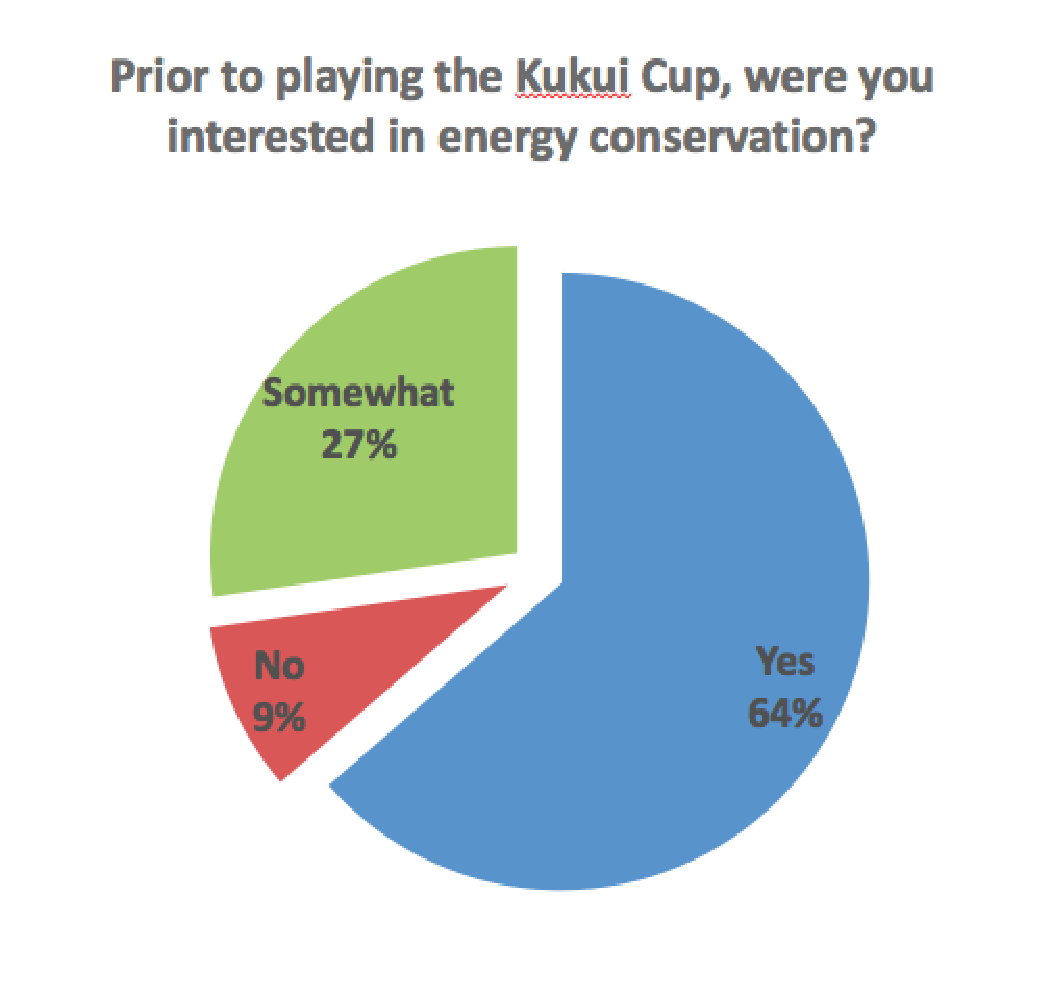
\includegraphics[height=2.2in]{effect-prior-2012.eps}}
		\subfigure[increased interests in sustainability after]{\label{fig:effect-after}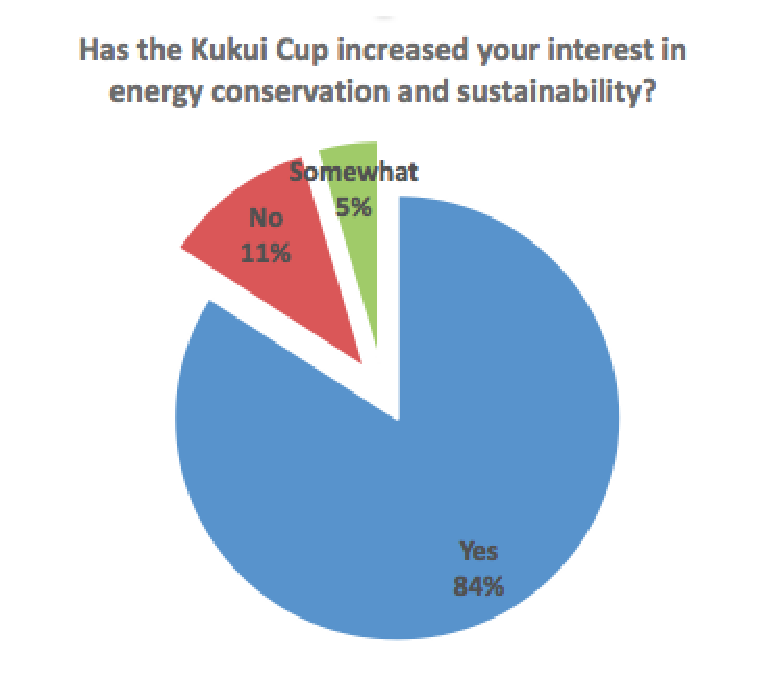
\includegraphics[height=2.2in]{effect-after-2012.eps}}
		\caption{Interests in Sustainability Prior and After the 2012 UHM KC}
		\label{fig:effect-prior-after-2012}
\end{figure}

The self-reported responses from 2012 KC indicates that there are a smaller percentage (9\%) of players than 2011 KC that were not interested in the sustainability prior to the Kukui Cup. After playing the Kukui Cup, 89\% of responses reported an affirmative or somewhat increase of interests in sustainability. There are 5 players (11\%)  reported that there is no changes of interests in sustainability. A closer look at the data indicates that the 5 players that reported no changes of interests also answered ``Yes'' or ``Somewhat'' interested to the sustainability prior to the Kukui Cup. The 4 players that reported no interests in sustainability also reported that playing KC had increased their interests.

The followings are some sample responses from the students who considered the Kukui Cup had increased their interests in sustainability:
 
 \begin{itemize}
 \item Yes. I'm more aware of everything I am using.
\item I've been interested, but the Kukui Cup has expanded and broadened my mind on what else I can be doing to help with conservation and sustainability. I think people are genuinely concerned, they just don't know how to exactly conduct them, or what other ways they can do it.
\item Yes, it made me realize that you can save a lot of money by turning off and unplugging a few things. (Hopefully lower tuition? =D )
\item It has increased my interest since I didn't know much about how much energy were using.
\item Some workshops made me think differently of how I use energy. Makes alternatives more interesting for me.
\item It taught me some new interesting facts about renewable energy and made me more aware.
\end{itemize}

There was a question in the 2011 KC survey tasking about the players' perception about how would they describe the Kukui Cup. The players were asked to check all that applies to their agreement to the following descriptions of the Kukui Cup: Educational, Fun, Addictive, So-so, Difficult, Boring, Not useful, and Other where they will type in their free text response. There were 43 responses from the 2011 KC survey. The number of responses and their percentage are listed in the \autoref{table:how-is-kc}.

\begin{table}[ht!]
  \centering
  \begin{tabular} {|c|c|c|}
    \hline
    \tabhead{Question: How would you describe the Kukui Cup?} & \tabhead{Number of Responses} & \tabhead{Percentage}\\
    \hline
Educational	& 41 & 95\%\\
    \hline
Fun	& 39 & 91\% \\
    \hline
Addictive	 &19 & 44\%\\
    \hline 
So-so	& 9 & 21\%\\
    \hline
difficult	& 3 & 7\%\\
    \hline
Boring	& 1 & 2\%\\
    \hline
not useful	& 0 & 0\\
    \hline
Other & 5 & 12\%\\   
    \hline 
  \end{tabular}
  \caption{Self-reported Perception of the Kukui Cup in 2011 UHM KC (n=43)}
  \label{table:how-is-kc}
\end{table}
	
Majority of the responses indicated the players perceived the Kukui Cup as ``Educational'' (95\%) and ``Fun'' (91\%). There are 44\% players perceived Kukui Cup as ``Addictive". On the other hand, there are 1 player (2\%) considered the Kukui Cup as``Boring". The ``Other'' responses are: ``AWSOME-NESS''(1), ``engaging''(1), ``fun competition''(1), ``Great way to bond with others''(1), ``impressive''(1).

A survey question was also asked about the players' self reported behavior change during the challenge in the 2012 UHM Kukui Cup. The question is ``Did you change your behavior during the competition based on the commitment(s) you made? if so, how?". It is a free response question. 45 players completed the survey in the 2012 UHM KC. I categorized the free text responses into three categories: ``Yes'', `already a habit'', and ``no''. The results are listed in \autoref{table:behavior-change}.

\begin{table}[ht!]
  \centering
  \begin{tabular} {|p{0.5\linewidth}|c|c|}
    \hline
    \tabhead{Question: Did you change your behavior during the competition based on the commitment(s) you made?} & \tabhead{Number of Responses} & \tabhead{Percentage}\\
    \hline
Yes	& 39 & 87\%\\
    \hline
Already a habit	& 4 & 9\% \\
    \hline
No	 &2 & 4\%\\
    \hline 
  \end{tabular}
  \caption{Self-reported Behavior Changes in 2012 UHM KC (n=45)}
  \label{table:behavior-change}
\end{table}

The examples of a ``Yes'' response are:
\begin{itemize}
\item ``I changed my behavior during the commitments but found myself doing the same things i did before after they were over.''
\item ``Yes, because knowing the facts of how much energy we use has helped me realize that I have been wasting money and energy.''
\item ``yes, my behavior has changed during the competition. I'm more aware of the things i do such as turning off appliances when not in use, as well as using more natural energy such as sunlight, rather than electricity.''
\end{itemize}

A ``Already a habit'' response is that the commitments already become part of the daily habit. The examples are:
\begin{itemize}
\item ``Most of the commitments I made I already did.''
\item ``I always turn off my lights when I leave the room, use cold water to wash my clothes, and I lessen my meat intake. ''
\end{itemize}

The self-reported survey results indicate in general, the players of Makahiki considered their experiences are positive and there had some self-reported impacts to their sustainability behaviors. 

\subsubsection{Self-reported usability survey}

A survey to gather the opinions of players regarding the usability of the website was added during the last round of the challenge. 

The players were asked to rate how much you agree with the following 4 usability statements in a likert scale (Strongly disagree, Disagree, Neutral, Agree, Strongly agree):
\begin{enumerate}
\item ``It was easy to find what I was looking for in the website.''
\item ``The website was responsive. I did not wait too long after I clicked on something.''
\item ``The website provided adequate help in teaching me how to play the game.''
\item ``I understood the rules of the game and how to play.''
\end{enumerate}

The questions were asked in both the 2011 and 2014 Kukui Cup in the University of Hawaii at Manoa, 43 players completed the survey in the 2011 KC while 18 players completed in the 2014 KC.  

\autoref{table:self-report-usability-2011}  and \autoref{table:self-report-usability-2014}  lists the results of the self-reported usability responses for both 2011 and 2014 Kukui Cup at UHM.

\begin{table}[ht!]
  \centering
  \begin{tabular} {|p{0.45\linewidth}|p{0.09\linewidth}|p{0.08\linewidth}|p{0.08\linewidth}|p{0.08\linewidth}|p{0.08\linewidth}|}
    \hline
    \tabhead{} & \tabhead{Strongly disagree} & \tabhead{Disagree} & \tabhead{Neutral} & \tabhead{Agree} & \tabhead{Strongly agree}\\
    \hline
It was easy to find what I was looking for in the website.& 2 & 1 & 2 & 14 & 24 \\
    \hline
The website was responsive. I did not wait too long after I clicked on something.& 2 & 1 & 1& 19 & 20 \\
    \hline
The website provided adequate help in teaching me how to play the game.	 & 1 & 1 & 1 & 16 & 24\\
    \hline
I understood the rules of the game and how to play	& 1& 1 & 0 & 12 & 29\\
    \hline 
  \end{tabular}
  \caption{Self-reported Usability in 2011 UHM KC (n=43)}
  \label{table:self-report-usability-2011}
\end{table}

\begin{table}[ht!]
  \centering
  \begin{tabular} {|p{0.45\linewidth}|p{0.09\linewidth}|p{0.08\linewidth}|p{0.08\linewidth}|p{0.08\linewidth}|p{0.08\linewidth}|}
    \hline
    \tabhead{} & \tabhead{Strongly disagree} & \tabhead{Disagree} & \tabhead{Neutral} & \tabhead{Agree} & \tabhead{Strongly agree}\\
    \hline
It was easy to find what I was looking for in the website.& 0 & 0 & 1 & 9 & 8\\
    \hline
The website was responsive. I did not wait too long after I clicked on something.& 0 & 4 & 2 & 10 & 2 \\
    \hline
The website provided adequate help in teaching me how to play the game.& 0 & 0 & 2 & 10 & 6 \\
    \hline
I understood the rules of the game and how to play.& 0 & 0 & 1 & 10 & 7 \\
    \hline 
  \end{tabular}
  \caption{Self-reported Usability in 2014 UHM KC (n=18)}
  \label{table:self-report-usability-2014}
\end{table}

\autoref{fig:self-report-usability-2011-2014} illustrates the self-reported usability measurements in both 2011 KC and 2014 KC. Majority of players reported that they agreed that the usability of the website is good with one exception of responsiveness from the 2014 responses. 4 out of 18 players (22\%) of 2014 KC reported that they considered the website is not very responsive. Comparing to the result of the 2011 KC, this indicates that there may be a perceived performance downgrade in the 2014 KC website.

\begin{figure}[ht!]
	\centering
		\subfigure[2011 Self-reported Usability Measurements(n=43)]{\label{fig:self-report-usability-2011}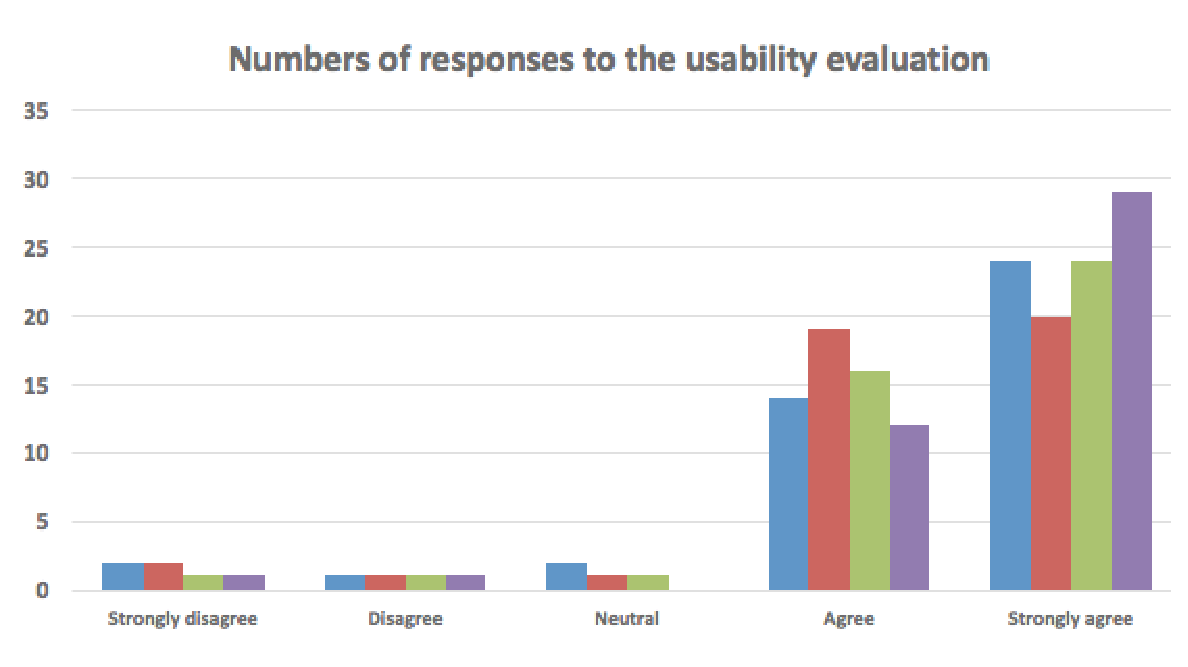
\includegraphics[height=3in]{self-report-usability-2011.eps}}
		\subfigure[2014 Self-reported Usability Measurements(n=18)]{\label{fig:self-report-usability-2014}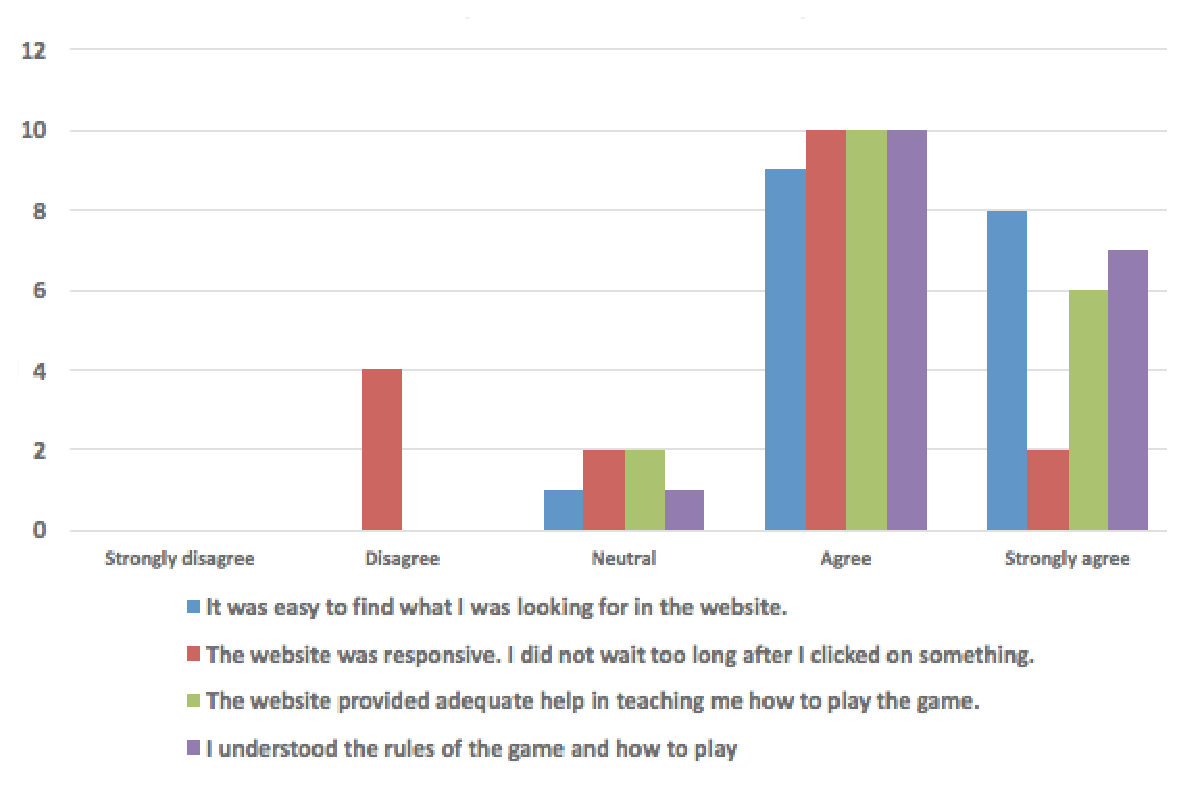
\includegraphics[height=3in]{self-report-usability-2014.eps}}
		\caption{Self-reported Usability Measurements in 2011 KC and 2014 KC}
		\label{fig:self-report-usability-2011-2014}
\end{figure}

Another question was asked in the 2014 UHM KC survey regarding the issues encountered when playing using the website. There are 3 out of 18 responses (17\%) reported that the loading of the website page were slow. This confirms the responsiveness issues discovered in the self-reported usability measurements described above. Another issues reported in the responses to the survey question is the confusion of the scoreboard display in the website. 3 out of 18 responses (17\%) reported that scoreboard's display keep changing so it is not easy to see their rankings. There are also 2 responses reported that some of the videos were not displayed which is due to the links to the videos were outdated.

In summary , the self-reported usability survey is a good tool to get feedback from the players of Makahiki to reveal the strengths and weaknesses regarding the usability of the game. 

\subsubsection{Engagement metrics}

Based on the engagement metrics \ref{Engagement metrics} proposed in the SGSEAM, we calculated a variety of engagement metrics to assess the player's engagement level in the Kukui Cup challenge created by the Makahiki framework. The metrics are calculated by analyzing the website logs and the data collected by the website. The results shown in \autoref{fig:makahiki-engagement} are the engagement metrics for the 2011 Kukui Cup challenge at the University of Hawaii at Manoa.
    
\begin{figure}[ht!]
  \centering
  \begin{tabular}{|l|c|c|c|c|c|c|}
    \hline
    \tabhead{\multirow{2}{*}{Measurement}} & \multicolumn{3}{c|}{\tabhead{2011 KC}} & \multicolumn{3}{c|}{\tabhead{2012 KC}}\\
     \cline{2-7}
    \tabhead{} & \tabhead{MIN} & \tabhead{AVG} & \tabhead{MAX} &  \tabhead{MIN} & \tabhead{AVG} & \tabhead{MAX}\\

    \hline
    Participation rate & 13\% & 37\% & 74\% & 19\% & 34\% & 64\%\\
    \hline
    Number of players per day & 43 & 85 & 147 & 0 & 12 & 130 \\
    \hline
    Play time per day & 1 min & 27.7 mins & 8.5 hours & 0 & 6.2 mins & 8.8 hours\\
    \hline
    Submissions per day & 32 & 266 & 1110 & 0 & 30 & 953\\
    \hline
    Social interactions per day & 51 &  208 & 468 & 0 & 31 & 502\\
    \hline
    Website errors per day & 0 & 0.6 & 4 & 0 & 2 & 458\\
    \hline
  \end{tabular}
  \caption{Engagement Metrics for 2011 and 2012 UHM Kukui Cup}
  \label{fig:makahiki-engagement}
\end{figure}

The participation rate is the percentage of players who played the game. The 2011 UHM KC had a 37\% average participation rate, while the 2012 KC had 34\%. Both are good compared to other sustainability challenges. 

Over the 3 weeks course of the challenge in the 2011 KC, an average player spent about 27.7 minutes per day on the website, while in the 24 weeks challenge in 2012 KC, an average player spent about 6.2 minutes per day. Both instances had one player spent over 8 hours (8.5 and 8.8 respectively) on one day, which is quite significant amount of time for a student to spent in this kind of game. The daily minimum time spent on the 2011 KC is 1 minute which indicates that for every day during the challenge, there are at least one player who played at least 1 minute. The daily minimum time spent on the 2012 KC is 0 minutes. This indicates that there are at least one day when no player use the website.

In order to investigate the engagement in a more details, we looked at the engagement measurement in a time series format. \autoref{fig:timeseries-metrics} shows the timed measurements graph during the 2011 and 2012 Kukui Cup.

\begin{figure}[ht!]
  \center
  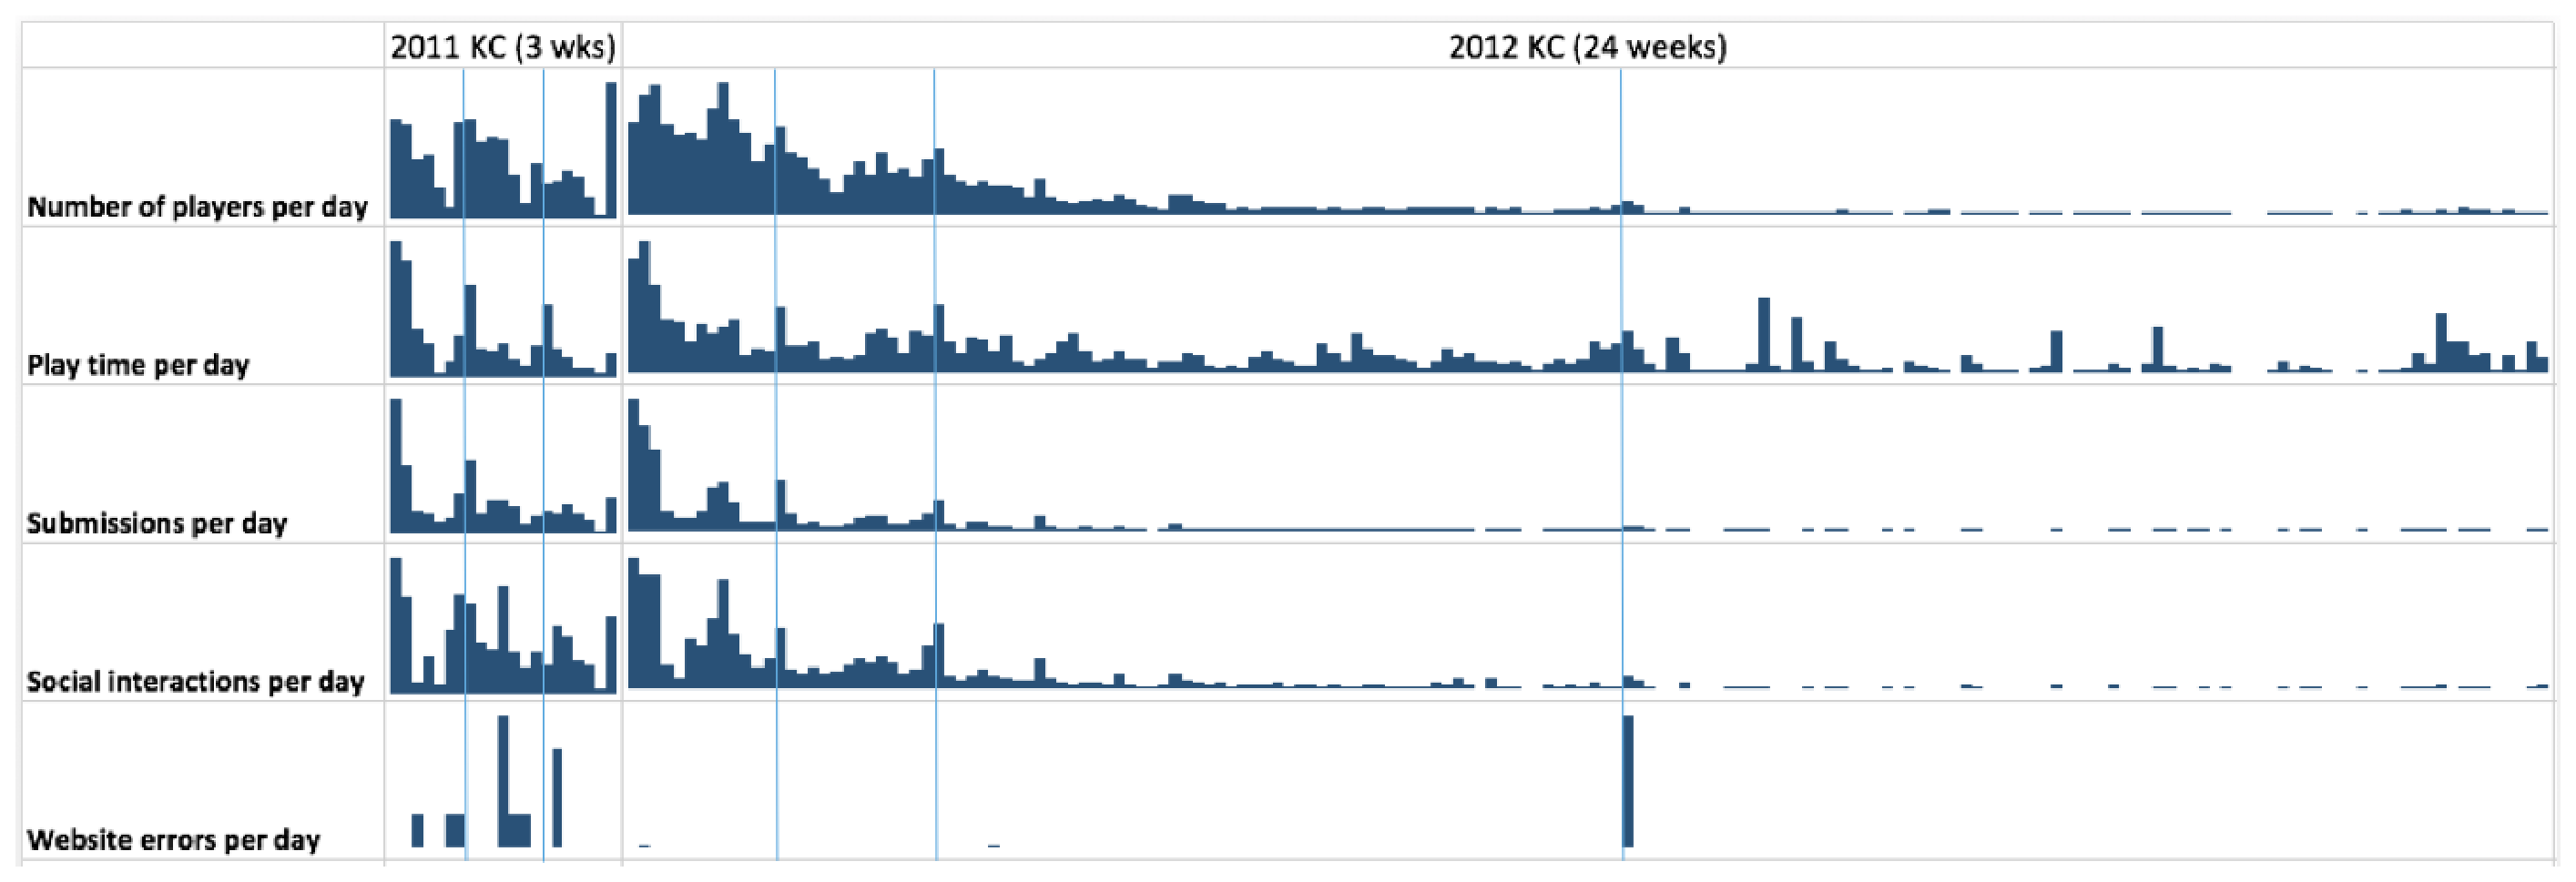
\includegraphics[height=3.2in,width=6.2in]{timeseries-metrics}
  \caption{Engagement Measurements during the 2011 and 2012 UHM Kukui Cup}
  \label{fig:timeseries-metrics}
\end{figure}

The divided line in the graphs indicates the division of the rounds for the 2011 and 2012 KC. In the 2011 KC, there are 3 rounds, each round lasted 1 week. In the 2012 KC, there are 4 rounds, the first and second round lasted 2 weeks each, and the third round lasted about 8 weeks, while the last round lasted about 12 weeks, with the total of 24 weeks for the 2012 KC. 

In addition to the daily number of players and daily play time which indicate the level of visits to the website or game, the daily submission and daily social interaction measurement indicate the level of deeper interactions with the game. We can see that during the 3 short weeks of the 2011 KC, the engagement patterns are similar in each week. The first few days has higher level of interactions then decreased later into the week. There is a spike on the last day of the round, which may be due to the urge of the players to check the winning results of the round. 

We can also see that in the 2012 KC, the engagement level significantly dropped after the second round, which is 4 weeks after the beginning of the game. There are still some numbers of players spent times on the game but the number of submissions and social interactions had decreased significantly. Over the time, the number of players decreased in the third round and even less in the last round. It is interesting to see that there are still some amounts of play time during the third and fourth round. A closer look at the data indicated that they are time spent from the the several top players who may be winning the game. 

Although the website error in the 2012 KC shown in the  \autoref{fig:makahiki-engagement} seems high, the detailed graph in \autoref{fig:timeseries-metrics} shows that the errors mostly happened during in one day which is the day after the start of the last round. The investigation of the error in the log file revealed that they are due to a content configuration error in a newly available event in the last round. The error caused the players not able to submit the completion of the event to claim their points so they kept trying and encountered the error repeatedly. The error was corrected 2 hours later after the first such error occurred.

In summary, SGSEAM indicates that Makahiki can be successful in achieving player engagement and literacy improvement. SGSEAM could not provide evidence of positive change in
behavior.

\subsection{Makahiki System Admin Assessment}
We used two approaches to assess the system administrators' experience with the Makahiki framework. They are in-lab installation study and post-hoc system admin interview.

\subsubsection{In-lab installation study}

In the in-lab installation study, the participants are the students in a serious game class (ICS691) in the Spring 2012 in the computer science department at the University of Hawaii at Manoa. The students were tasked with installing the Makahiki system into their local computers as well as deploying to the Heroku cloud environment. A Google Form was used to ask the students to record the time they spent completing each step and the problems they encountered. The students also provided feedback about their installation experiences in the form of blog posts. 

The results from the Google Form responses show that the average total time to successfully install
Makahiki was 1.4 hours, with a maximum time of 2 hours and the minimum time of 0.9 hour.
\autoref{fig:install-time} shows the average time for each installation step.

\begin{figure}[ht!]
  \center
  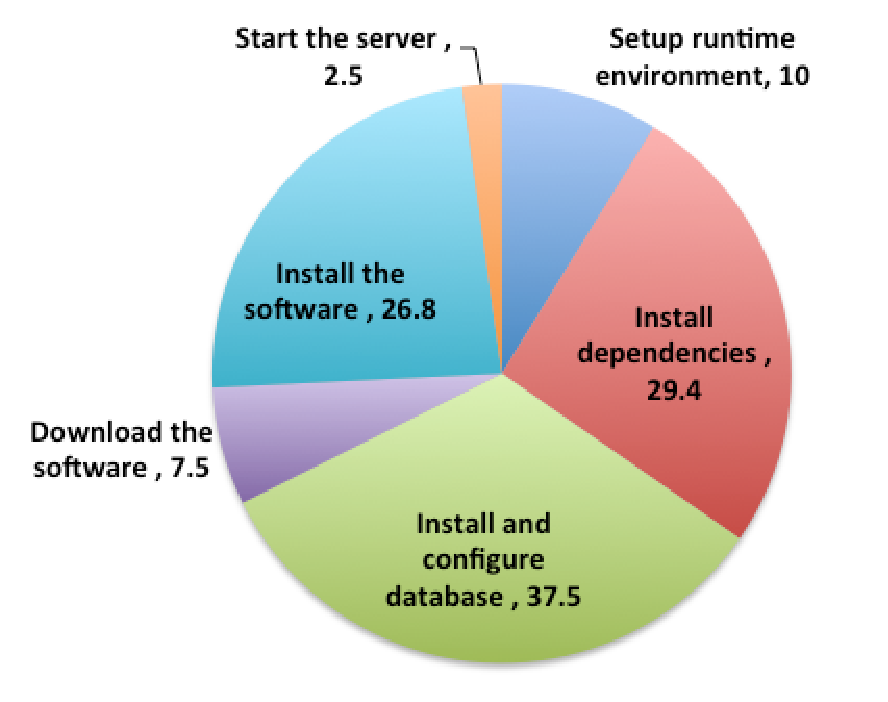
\includegraphics[width=0.7\columnwidth]{install-time}
  \caption{Average time (minutes) for installation steps (n=8)}
  \label{fig:install-time}
\end{figure}

We coded and categorized the descriptive problems reported by the students in both the Google Form
and their blog posts. \autoref{fig:makahiki-install} shows the result of the analysis from
the feedback of the 8 students that participated in the experiment.

\begin{figure}[ht!]
  \centering
  \begin{tabular}{|c|c|}
    \hline
    \multicolumn{1}{|p{0.7\columnwidth}|}{\centering\tabhead{Problem encountered}} &
    \multicolumn{1}{|p{0.2\columnwidth}|}{\centering\tabhead{Number of participants}} \\
    \hline
    \multicolumn{1}{|p{0.7\columnwidth}|}{Cannot find configuration file to edit during database installation } &
    \multicolumn{1}{|p{0.2\columnwidth}|}{4} \\
    \hline
    \multicolumn{1}{|p{0.7\columnwidth}|}{Documentation of install script is confusing about creation of the DB user} &
    \multicolumn{1}{|p{0.2\columnwidth}|}{2} \\
    \hline
    \multicolumn{1}{|p{0.7\columnwidth}|}{More parts of installation could be covered by install script} &
    \multicolumn{1}{|p{0.2\columnwidth}|}{2} \\
    \hline
  \end{tabular}
  \caption{Makahiki Installation Analysis (n=8)}
  \label{fig:makahiki-install}
\end{figure}


From the above analysis, we identified that the ``Install and configure database'' step has the
longest average time. It is also has the most participant reported problems. This reflects the issues
encountered by students during the configuration process. This assessment determines the areas for future
improvement are (1) to improve documentation on DB installation, and (2) to improve the install script to automate
more installation tasks.

In summary, SGSEAM identified database installation as a weak point in
installation.  Otherwise, SGSEAM indicates generally positive results regarding
Makahiki with respect to installation.

\subsubsection{Post-hoc System Admin Interview}
In order to gain insights on the experience of a real world system admin who uses the Makahiki, I performed interviews to the system admins of the Hawaii Pacific University (HPU) Kukui Cup challenges. The interview questions are outlined in the system admin assessment section of the SGSEAM. The interview took place after the challenge. Before the challenge, the system admin performed the installation of the Makahiki in the HPU local infrastructure. Issues encountered during the installation were communicated through emails and phone calls. They are recorded and analyzed as well as the interview data.

I analyzed qualitative data collected from the interviews and email changes. The data include: � time taken to install the Makahiki
� time taken to maintain the Makahiki, such as backup, monitoring
� problems encountered

\subsection{Makahiki Game Designer Assessment}

\subsubsection{In-lab game design study}

We also used the in-lab experiment to assess the game
designer experience of Makahiki. One of the class assignments for the students in the
experiment was to design a serious game using the Makahiki framework. We asked the students
to follow specific design steps and record the time required and any problems encountered during
their design process, using a Google Form similar to the one used for the system admin
assessment. In addition, students were asked to provide feedback about their
design experiences in the form of blog posts. \cite{csdl2-13-04} describes in detailed
the Google Form that is used in this assessment.

The game designer assessment was generalized into 7 tasks corresponding to
distinct types of administrative tasks and game design planning. The time for each task is
calculated from the Google Form results.  The most time consuming task
 is "Smart Grid Game Design", which took average 107.9 minutes (56\% of total time) to complete,
 while the least time
  consuming tasks is "Raffle Game Design", which took average 7.9 minutes (7\% of total time)
  to complete.

\autoref{fig:design-time} shows the average time for each design tasks:

\begin{figure}[ht!]
  \center
  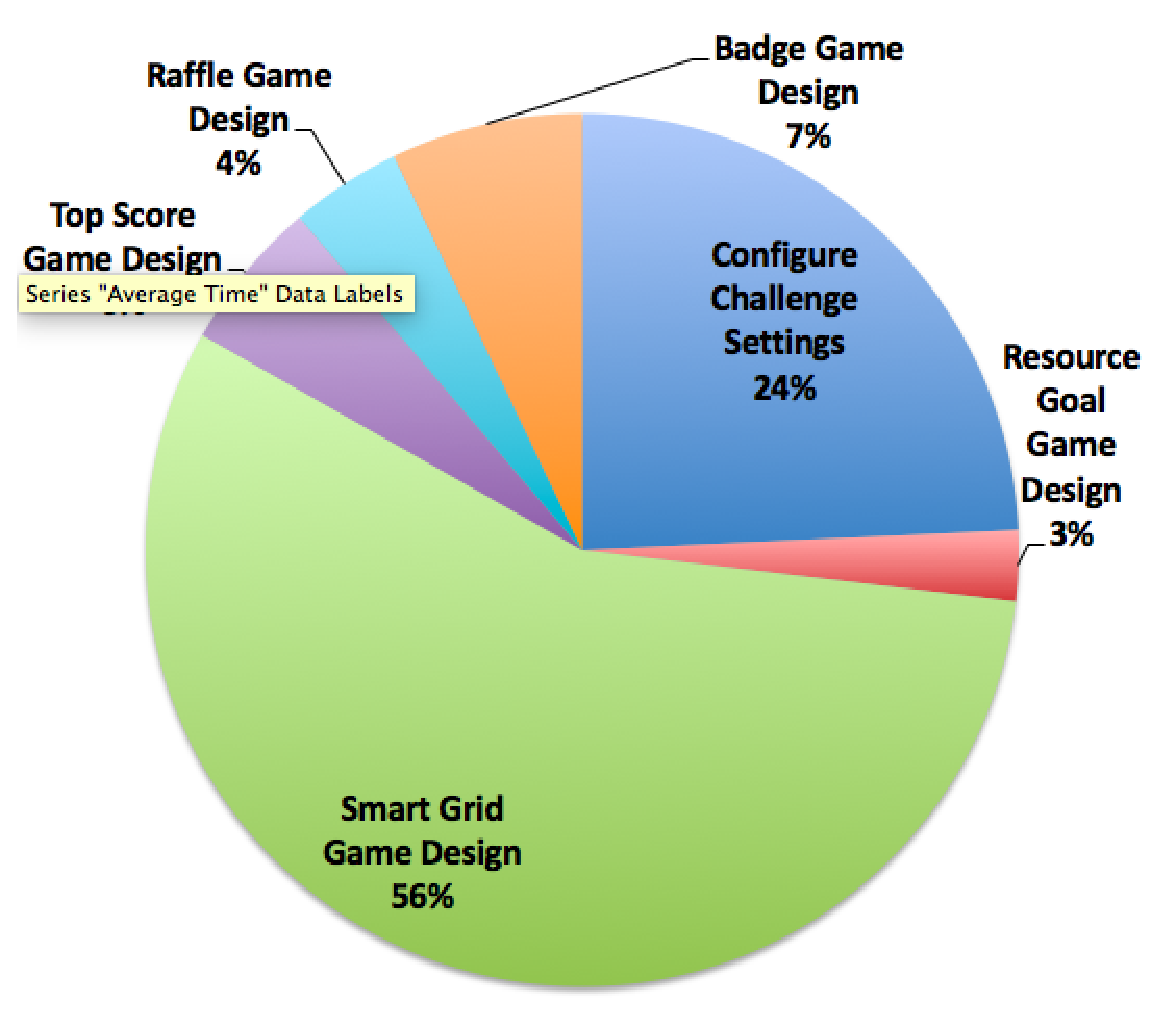
\includegraphics[width=0.7\columnwidth]{design-time}
  \caption{Average time (minutes) for design tasks (n=8)}
  \label{fig:design-time}
\end{figure}

 We aggregated the problems reported in the feedback of the 7 students that participated in the experiment.
\autoref{fig:makahiki-game-design} shows the result of the analysis:

\begin{figure}[ht!]
  \centering
  \begin{tabular}{|c|c|c|}
    \hline
    \multicolumn{1}{|p{0.7\columnwidth}|}{\centering\tabhead{Problem encountered}} &
    \multicolumn{1}{|p{0.2\columnwidth}|}{\centering\tabhead{Number of participants}} \\
    \hline
    \multicolumn{1}{|p{0.7\columnwidth}|}{Difficulty in understanding predicate system and unlock condition} &
    \multicolumn{1}{|p{0.2\columnwidth}|}{7} \\
    \hline
    \multicolumn{1}{|p{0.7\columnwidth}|}{A bug that prevented users with usernames
containing capital letters from logging in} &
    \multicolumn{1}{|p{0.2\columnwidth}|}{2} \\
    \hline
    \multicolumn{1}{|p{0.7\columnwidth}|}{A bug in the processing of Ajax queries} &
    \multicolumn{1}{|p{0.2\columnwidth}|}{1} \\
    \hline
    \multicolumn{1}{|p{0.7\columnwidth}|}{Difficulty in generating event attendance codes for game activities} &
    \multicolumn{1}{|p{0.2\columnwidth}|}{1} \\
    \hline
  \end{tabular}
  \caption{Makahiki Game Design Analysis, (n=8)}
  \label{fig:makahiki-game-design}
\end{figure}

In summary, SGSEAM revealed two shortcomings with Makahiki configuration: ``Smart
Grid Game Design'' and ``Configure Challenge Settings''. Issues encountered in ``Smart Grid Game
Design'' included 1) difficulty and lack of documentation on the predicate system used to define dependencies
between game activities, and 2) difficulty in generating event attendance codes for game activities.
Issues encountered in ``Configure Challenge Settings'' included 1) a bug in the processing of Ajax queries
caused by consecutive clicks on the same interface button, and 2) a bug that prevented users with username
containing capital letters from logging in.

\subsection{Makahiki Game Manager Assessment}
We used the 2012 Kukui Cup Challenge at the Hawaii Pacific University (HPU) to assess
the game manager experience of Makahiki. We interviewed the
game manager of the HPU Kukui Cup challenge, who is also the game designer of the challenge.
We asked him about his game management experiences using the Makahiki admin
interface. The interview questions are outlined in the game manager section of the SGSEAM.

The interview took place after the challenge and was audio-recorded. We transcribed the
audio recording. The data shows that the game management interface was easy for him to use.
He made sure that player submissions were either approved or rejected
within 12 hours. He also discovered a useful feature in the approval interface without
help from the Makahiki support team. The only problem he reported was that after the
competition ended, he discovered that some of the analytics data disappeared. This was
identified by the Makahiki development team as a software bug and has since been fixed.

In summary, SGSEAM uncovered few problems with Makahiki game management using the interview
approach. We realized that the confident level of this assessment approach is low because of
 availability of only one data point. An experimental study approach or perform interviews to
multiple game managers will increase the confidence level of the assessment.

\subsection{Makahiki Developer Assessment}

We assessed developer experience using an in-lab experiment. One of the class assignments
for the students in the experiment was to develop an enhancement to Makahiki.  This
involved setting up a development environment, following the tutorial to create a ``Hello
world'' widget using Makahiki, and finally, developing an enhancement to extend the
functionality of Makahiki.

The students were asked to submit their development source code to the
public source code repository (GitHub) and write a blog post to
discuss their efforts to complete the development activity.

All 8 students reported that the first task of creating the simple ``Hello world'' widget
was easy, while the enhancement development was hard. Only one student successfully
completed all 5 required features, while the rest successfully completed 1 or 2
features. The main problem students reported was the lack of documentation for the
development libraries. One student stated in his blog that he decided to choose Makahiki
framework to develop his own serious game because of Makahiki's features and possibility
of reducing development effort by using the framework.

In summary, SGSEAM reveals significant problems with developer efficiency.
Analysis is still ongoing regarding the specific causes of problems and how best to
address them.
    
\section{Conclusions/Future Directions}

Our experiences thus far with the Makahiki+WattDepot software stack have shown it to be a
reliable and performant system for the provision of sophisticated energy challenges to
address the need for informed consumers in the development of the Smart Grid.

One future direction involves the development of a consortium of local organizations in
order to explore the use of this software stack in new settings.  This will create
challenges at both the design and implementation levels.   Moving outside of the context
of either Hawaii or college-aged users will necessitate development of significant new
forms of content, including activities, workshops, events, and videos. This challenge,
while significant, does not necessitate significant changes to the Makahiki+WattDepot
software stack.

A far more challenging future direction is an island-wide Kukui Cup, in which all of the residents of
Oahu would be able to login to the system and play the game. This creates challenges on
multiple levels: providing content appropriate to the user (an elementary student should
have activities different from her mother and father), obtaining energy data for
residential users from the local utility in a manner appropriate for the challenge and
interface this data with the system, and finally resolving the scalability problem
identified in the last section.  We will require the engagement of multiple stakeholders
from across the community spectrum to identify and resolve these issues. 



  

\bibliographystyle{plain}
\bibliography{/group/csdl/bib/psp,/group/csdl/bib/ftr} 


\end{document}



